%vormatierung
\documentclass[10pt,a4paper,bibliography=totocnumbered,listof=totocnumbered]{scrartcl}
%zeilenabstand
\usepackage{setspace}
\linespread{1.5}
%\onehalfspacing
\parindent 0pt

\usepackage{tabularx}
\usepackage[utf8]{inputenc}
%font änder
\usepackage[ngerman]{babel}
\usepackage[T1]{fontenc}
\usepackage{uarial}
\renewcommand{\familydefault}{\sfdefault}
\usepackage{blindtext}
%ränder
\usepackage[paper=a4paper,left=40mm,right=30mm,top=25mm,bottom=25mm]{geometry} 
%Abstand Fusnoten
\deffootnote{1em}{1em}{\textsuperscript{\thefootnotemark\ }}
%sub und subbubsection tiefe
\setcounter{tocdepth}{3}
%Inhaltsverzeignis anklickbar.
\usepackage{hyperref}
\setcounter{secnumdepth}{3}
%sonderzeichen
%\usepackage[T1]{fontenc}
%grafiken einbinden
\usepackage{graphicx}
\usepackage{pdflscape}
\usepackage{listings}
%\usepackage[none]{hyphenat}
\usepackage[backend=biber,style=alphabetic,]{biblatex}
\usepackage{biblatex}
\addbibresource{ref.bib}
\bibliography{ref.bib}
%\bibliographystyle{apalike} 
%\bibliographie{ref}



%Wie können künstliche Intelligenzen bei der Entwicklung eines Videospiels in der Unreal Engine 5 eingesetzt werden?
\title{Entwicklung eines Videospielprototypen als ,,Ein-Mann-Videospielentwickler´´ auf der Unreal Engine 5 mit Hilfe von KI-Systemen}

\author{Nicolas Taylor}

\date{11.04.2023}

\begin{document}
\thispagestyle{empty}
\begin{center}
		 
		 \vspace*{1cm}
		 \Large
		 \textbf{Hochschule Fulda}\\
		 \textbf{Fachbereich Angewandte Informatik}\\
		 \vspace*{4cm}
		 
		 \huge
		 \textbf{BA}\\
		 \vspace*{0.5cm}
		 \large
		 
		 \textbf{Entwicklung eines Videospielprototypen als Ein-Mann-Videospielentwickler auf der Unreal Engine 5 mit Hilfe von KI-Systemen}\\
		 \vspace*{1cm}
%	 \includegraphics[scale=1.0]{Bilder/logo.png}\\
%		 \vspace*{2cm}
		 
		 \vfill
		 \normalsize
\newcolumntype{x}[1]{>{\raggedleft\arraybackslash\hspace{0pt}}p{#1}}
   		 \begin{tabular}{x{6cm}p{7.5cm}}
               		 \rule{0mm}{5ex}\textbf{Autor:} & Nicolas Taylor - nicolas.taylor@gmx.net
               		 \\
               		 \rule{0mm}{5ex}\textbf{Prüfer:} & Prof. Dr. Christian Fischer
               		 \\
               		 \rule{0mm}{5ex}\textbf{Zweitprüfer:} & Dipl.-Ing. Peter Klingebiel
               		 \\
               		 \rule{0mm}{5ex}\textbf{Abgabedatum:} & 09.10.2023
               		 \\
   		 \end{tabular}
\end{center}
\pagebreak
\tableofcontents
\newpage
%1
\section{Einleitung}
"Sprechen Sie einfach diese magischen Worte aus: Ich bin ein Game Designer. (...) Haben Sie es gemacht? Wenn ja, dann gratuliere ich Ihnen. Sie sind jetzt ein Game Designer."\cite[S. 37]{schell2020kunst}
\\
Dieses Zitat stammt von Jesse Schell; Hochschullehrer für Unterhaltungstechnologie am Entertainment Technology Center in Pittsburgh, USA.
\\
Wenn er gefragt wird, was er macht, um seine Brötchen zu verdienen, antwortet er: "Ich bin Game Designer". Jesse Schell, ermutigt Anfänger in seinem Buch, die noch vor Ihrem ersten Schritt Game Designer oder Videospiele Entwickler stehen, sich selbst als Gamedesigner zu bezeichnen. Wenn wir den Worten von Jesse Schell Glauben schenken, ist Gamedesigner werden nicht schwer.
\\
Wenn man sich dazu entscheidet Videospiele zu entwickeln, stehen oft nur drei Wege zur Verfügung. Der erste Weg ist es in einem Großen Videospielentwicklungsstudium zu arbeiten die mehrere Hundert Angestellte haben. In diesen Studios ist es üblich mit einem sehr kleinen Aufgabenbereich beschäftigt zu sein. Der zweite Weg ist in einem kleinerem Entwicklerstudio anzufangen wo sich die Rollen in der Videospielentwicklung mit anderen aus dem Team Überschneiden. Der Vorteil in diesen beiden Wegen ist, das ein Entwickler von anderen Erfahreren Entwickler lernen kann. Der dritte und letzte Weg ist der Weg als Ein-Mann-Videospielentwickler. Als Ein-Mann-Videospielentwickler ist man gezwungen alle Aufgaben zu übernehmen die Anfallen um ein Videospiel zu entwickeln.
\\
In dieser Arbeit möchte ich mich mit der Frage auseinandersetzen wie KI-Systeme in der Entwicklung eines Videospiels unterstützen kann. Ich werde diese Frage als Ein-Mann-Videospielentwickler nachgehen und im Rahmen dieser Bachelorthesis ein Prototyp entwickeln und in meinem Projekt so viele KI-Systeme einbinden wie es Möglich und Sinnvoll ist.

%https://dailygame.at/baldurs-gate-3-entwickler-bleibt-weiterhin-unabhaengig/ -03.09.2023
 
\subsection{Motivation und Idee}
Videospiele werden aus sehr vielen Teilbereichen der Medienbranche zusammengesetzt, wie zum Beispiel Autoren, Programmierer und Illustratoren bis hin zu Marketing und Vertrieb.
\\
Die Vergangenheit hat merfach bewiesen das Videospiele von einer Person entwickelt werden könne. Spiele wie Stardew Valley das von Eric Barone entwickelt wurde, Minecraft das ursprünglich von Markus „Notch“ Persson entwickelt wurde oder Undertale das von Toby Fox entwickelt wurde.
\\
Spätestens in den 90er Jahren wurden nur noch sehr wenige Spiele von einer Person entwickelt die in Arcadehallen oder Kaufhäußer zugänglich waren.
Warum der Ein-Mann-Videospieleentwickler immer seltener wurde, liegt großteil daran, dass die Technik auf denen die Vidoepiele liefen mit der Zeit leistungsfähiger wurden und somit größere und Komplexere Spielewelten erschaffen konnten.
\\
Diese Komplexität der Spielewelten konnte nicht mehr von einem einzelnen Entwickler gewährleistet werden.
\\
Im Jahr 2022 hat die Firma OpenAI sein KI-Werkzeug ChatGPT der Öffentlichkeit zugänglich gemacht, und viele Berichte über einen Meilenstein in der KI-Forschung.
\\
ChatGPT kann selbständig durch eine für den Menschen einfache Prompt Schulaufgaben lösen oder sich mit dem Benutzer unterhalten.
\\
ChatGPT kann ganze Programme in verschiedenen Programmiersprachen Schreiben, was es davor nie in solchen Umfang da gewesen war.
\\
KI-Systeme bieten ein neues Gebiet um Forschung und Experimente zu betreiben, und ich möchte in meiner Bachelorthesis herausfinden ob es möglich ist, ein Videospiel mit hilfe von KI-Systemen zu entwickeln, so wie in der Pionierzeit wo einzelne Entwickler ganze Projekte erschaffen haben.
\\

 
Die Systeme, auf denen Videospiele liefen, wurden immer leistungsfähiger, und somit wurden auch lebendigere und komplexere Welten möglich. Videospiele wurden in der Regel nicht mehr von einer Person entwickelt, sondern von ganzen Studios. In diesen Studios werden Aufgaben auf Teams verteilt, wie zum Beispiel Concept Art and Design, Musik und Soundeffekte bis hin zum Vertrieb und Marketing.
\\
Kurz, ein Videospiel zu entwickeln ist schon sehr lange keine Ein-Mann-Aufgabe mehr, Und in solchen Teams kann jeder Videospielentwickler sich auf seine Stärken im Team konzentrieren.
\\
Ich sehe seit 2022 eine neue Möglichkeit Videospiele zu entwickeln, die zuvor in diesem Umfang nicht möglich gewesen war.
\\
KI-Systeme sind Werkzeuge, die ein hohes Potenzial beinhalten, um schnelles und qualitatives Arbeiten mit sich bringen.
\\
Mit Midjourney kann ich innerhalb von wenigen Minuten eine Landschaft erstellen lassen. ChatGPT kann dir Geschichten schreiben und Voice.ai dir eine neue Stimme verleihen. Das was die vorhin drei genannten KI-Systeme sich spezialisiert haben, sind in der realen
Welt, echte Berufe in der Gamingbranche - Concept Artist, narrative Designer / video game writer, voice actor.
\\
Es ist heute theoretisch möglich, ohne viele Vorkenntnisse diese Aufgaben mit Hilfe von KI-Systemen zu übernehmen.
\subsection{Forschungsfrage}

\subsection{Forschungsmethoden}
Ich werde in dieser Arbeit einen Prototyp entwickeln. Während dieser Arbeit werde ich versuchen, Probleme und Aufgaben mit KI-Systemen zu lösen. Diese Lösungen werde ich in dieser Arbeit präsentieren.
\subsection{Gliederung der Arbeit}%todo hööööö?!
Die Arbeit ist gegliedert in, Warum ich was mache, dann ein Paar allgemeine Erklärungen.
\\
Was ich mache. Und welche Werkzeuge ich benutze. Ich werde Alles am Ende analysieren
\subsection{Zielsetzung}
Mein Ziel in dieser Arbeit ist es, einen Prototyp zu entwickeln. Dieser Prototyp wird nur von einer Peron entwickelt, und alle anderen Aufgaben und Probleme werden versucht, mit Hilfe von KI-Systemen zu lösen.
\subsection{Abgrenzung}
\section{Fragestellung}
KI ist ein großes Technologiefeld, was schon seit 15 Jahren daran geforscht wird. Seit ChatGPT 2022 für die breite Öffentlichgkeit geöffnet wurde, ist ein Bewustsein für diese Technologie geschaffen wurden.
\\
Viele gesellschaftliche, und industrielle gebiete sind oder werden in nahe zukunft mit KI-Systemen ihren Alltag finden.
\\
Viele KI-Systeme können mittlerweile sehr kreative Aufgaben sehr schnell bearbeiten und Resultate hervorbringen.
\\
Bilder, Stimmen, Animationen, Text. Alles Medienformen die in Videospiele benötigt werden um ein Fertiges Produkt zu erzeugen.
\\
Wie weit kommt Stand Heute ein Ein-Mann-Videospieleentwickler, wenn er sich dieser KI-Systeme bedient? Was sind die Hürden? Was sind die Vorteile? Ist es sinnvoll, auf solche Systeme zurückzugreifen, um einen Prototypen zu entwickeln.
\\
Diese Fragen möchte ich in meiner Bachelorthesis klären.
\\
Ich werde selber forschen, welche KI-Systeme es gibt und welche ich wie und in welcher Weise ich benutzen kann, um ein Prototypen zu entwickeln.
 
\section{Theoretischer Hintergrund}
%\\\\\\\\\\\\\\\\\\\\\\\\\\\\\\\\
\subsection{Begriffsdefinitionen}%erläuterung
%\\\\\\\\\\\\\\\\\\\\\\\\\\\\\
\subsubsection{KI-System}
%https://www.bsi.bund.de/DE/Themen/Verbraucherinnen-und-Verbraucher/Informationen-und-Empfehlungen/Technologien_sicher_gestalten/Kuenstliche-Intelligenz/kuenstliche-intelligenz_node.html
Mittels maschinellen Lernens großer Datenmengen, können KI-Systeme, selbständige Lösungskompetenzen erwerben. KI-Systeme können die Fähigkeit besitzen, Eingabedaten, die nicht zu ihren Trainingsdaten vorkommen, zu verarbeiten.
\subsubsection{Prompt}
%https://dict.leo.org/englisch-deutsch/prompts ; https://bm-experts.de/definitionenfaq/definitionen/prompt-was-ist-das-und-wie-kann-er-eingesetzt-werden/
Aus dem Englischen, to prompt, und bedeutet so viel wie auordern oder ab fragen. Der User benutzt Prompts, um einem KI-System einen Befehl zu überreichen. Im Beispiel von ChatGPT gibt der User ein Prompt in das Chatfenster, undb ChatGPT generiert eine passende Antwort.
\subsubsection{NPC}
% (DKDG) Klaus Breuer - Computerspiele programmieren - Künstliche Intelligenz für Künstliche Gehirne - Kapitel 15.1 Erster Absatz Seite 113 ------ Computerspiele programmieren: künstliche Intelligenz für künstliche Gehirne / Breuer, Klaus Barcode 12155751 Rückgabe bis 12.06.2023
Non-Player Characters, kurz NPC, sind vom Computer gesteuerte Charaktere, Dorfbewohner, Tiere oder Monster. Alle Charaktere und Tiere, die sich nicht vom Spieler kontrollieren lassen. NPCs sind notwendig, um eine Spielwelt lebendig wirken zu lassen.
\subsubsection{Game Designer}
%Die Kunst des Game Designs : bessere Games konzipieren und entwickeln / Schell, Jesse Barcode 12486880 Kapitel 1.2 Seite 35 bis 37 DKDG
Ein Game Designer besitzt ein breites Spektrum an Fähigkeiten wie Animation, Architektur, Betriebswirtschaft, Game Engineering, Darstellende Kunst, Geschichte, Management, Mathematik, Musik, Präsentation, Soundgestaltung, Spiele und viele weitere beherrschen sollte.
\\
Der Game Designer erschafft ein Erlebnis, wobei das Spiel nicht das Erlebnis ist, sondern nur die Möglichkeit, dem Spieler ein Erlebnis zu erleben.
%Kapitel 2.1 Seite 44
\subsubsection{Design}%Seite 49 oder eine andere gemeingültige Quelle DKDG
\subsubsection{Spiel}%Kapitel 4.2 seite 74 bis 89-- Großes Kapitel
\subsection{Videospiel-Entwicklung}
\subsubsection{Die Vier Grundelemente eines Videospiels}%Kapitel5.2 Seite 93 DKDG
\subsection{Unreal Engine 5}
%https://www.unrealengine.com/de/unreal-engine-5 abrufdatum 27.05.2023
Die Unreal Engine ermöglicht den Spieleentwickler 3D-Videospiele zu entwickeln. Die Entwicklung eines Videospiels in der Unreal Engine 5 kann in Echtzeit entwickelt werden, das bedeutet, dass man das Ergebnis seiner Arbeit sofort betrachten kann. Epic Games, die Entwickler der Unreal Engine 5, beschreiben sie als "Das weltweit offenste und fortschrittlichste Tool zur 3D-Erstellung in Echtzeit".
\subsubsection{Narnite}
\subsubsection{Lumen}
\subsection{Künstliche Intelligenz und ihre Anwendungen in der Videospiel-Entwicklung}
\subsection{Vor- und Nachteile des Einsatzes von KI in der Videospiel-Entwicklung}
%3
\section{Methodik}
\subsection{Auswahl und Beschreibung der KIs}
\subsubsection{ChatGPT}
\subsubsection{Midjourney}
\subsubsection{PIFuHD}
\subsubsection{Voice.AI}
\subsubsection{Adobe Enhanced Speech}
\subsection{Beschreibung der Tools und Technologien}
\subsubsection{Blender}
\subsubsection{Audacity}
\subsection{Beschreibung des Entwicklungsprozesses}
%4
\section{Umsetzung}
\subsection {Idee und Konzeption}
Meine Idee ist ein Videospiel zu entwickeln, das eine geschichtliche und kulturelle Relevanz zur deutschen Geschichte hat. Ein weiteres Kriterium an meinem Videospiel ist es, ein Szenario zu wählen, das sich vor dem Zweiten Weltkrieg befindet. Mit dieser Idee habe ich folgenden Prompt für ChatGPT formuliert und anschließend dien in Abbildung \ref{ersten-5-themen}Ausgabe bekommen.
\begin{figure}[h]
   		 \centering
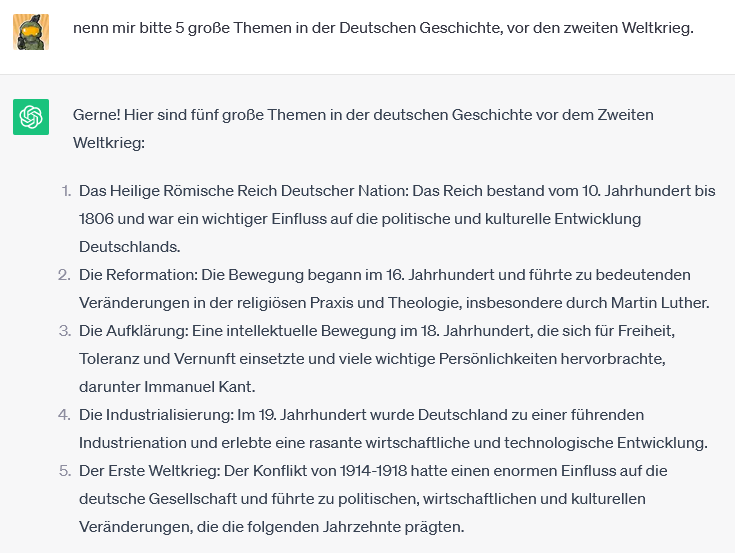
\includegraphics[width=14cm]{BilderFuerBA/CGPTBachelorarbeitZurKI/01.png}
   		 \caption{Ersten fünf Themen}
   		 \label{ersten-5-themen}
\end{figure}
\\
Nachdem ich mit den ersten 5 Ideen von ChatGPT nicht zufrieden habe ich mir weitere 5 Themen ausgeben lassen die in Abbildung \ref{zweiten-5-themen}.
\begin{figure}[h]
   		 \centering
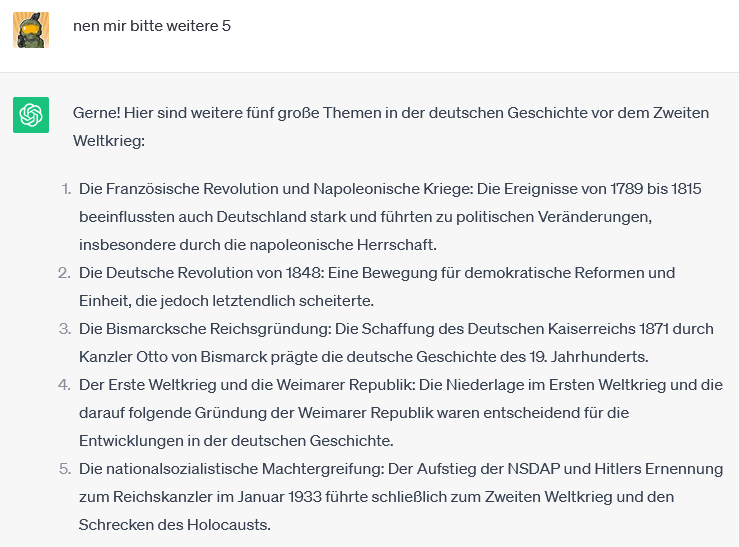
\includegraphics[width=14cm]{BilderFuerBA/CGPTBachelorarbeitZurKI/02.png}
   		 \caption{ChatGPT: Zweiten fünf Themen}
   		 \label{zweiten-5-themen}
\end{figure}
Man kann an diesem Beispiel sehen, dass ChatGPT mir 10 Ideen präsentiert, die ich in meinem Videospiel verarbeiten kann.
\\
Als Ein-Mann-Videospielentwickler entschied ich mich für die Reformation mit Martin Luther als Hauptfigur.
\\
Innerhalb dieser Bachelorthesis ist es mir aus Zeitgründen nicht möglich ein komplettes Videospiel zu entwickeln, was das Leben von Martin Luther widerspiegelt. Durch meine Recherche über Martin Luther und sein Leben fand ich den Moment bedeutend wo Martin Luther seine 96 Thesen an das Kirchtor nagelt.
\\
In meinem Prototyp werde ich dieses Ereignis als Thematischen Mittelpunkt wählen.
\\
Meine Spielidee für meinen Prototyp ist nun, dass Martin Luther durch ein Dorf läuft, verschiedene NPCs trifft und mit ihnen in einen Dialog tritt. Martin Luther trifft verschiedene Personen mit verschiedenen Problemen und Ansichten. Er redet mit ihnen und lässt sich von ihnen inspirieren. Durch diese Inspiration entwickelte Martin Luther später im Spiel, seine 96 Thesen.
\\
Kern des Prototyps ist die Entwicklung einer Spielwert, die aus einem Dorf mit verschiedenen Häusern und NPCs besteht.
\\
Die Entwicklung des Prototyps unterteilt sich in verschiedene Meilensteine:
-Hauptfigur
\\
-Landschaft
\\
-Gebäude
\\
-Nebenfiguren
\\
-Dialogsystem
\\
-Sprachausgabe
\\
Jeder dieser Meilensteine besitzt in dieser Theses sein eigenes Kapitel, in dem die Entwicklung nahegebracht wird.

%\\\\\\\\\\\\\\\\\\\\\\\\\\\\\\\\\\\\\\\\\\\\\\\\\\\\ HUPTFIGUR\\\\\\\\\\\\\\\\\\\\\\\
%\\\\\\\\\\\\\\\\\\\\\\\\\\\\\\\\\\\\\\\\\\\\\\\\\\\\ HUPTFIGUR\\\\\\\\\\\\\\\\\\\\\\\
%\\\\\\\\\\\\\\\\\\\\\\\\\\\\\\\\\\\\\\\\\\\\\\\\\\\\ HUPTFIGUR\\\\\\\\\\\\\\\\\\\\\\\
\subsection {Meilenstein: Hauptfigur}
\begin{figure}
	 \centering
	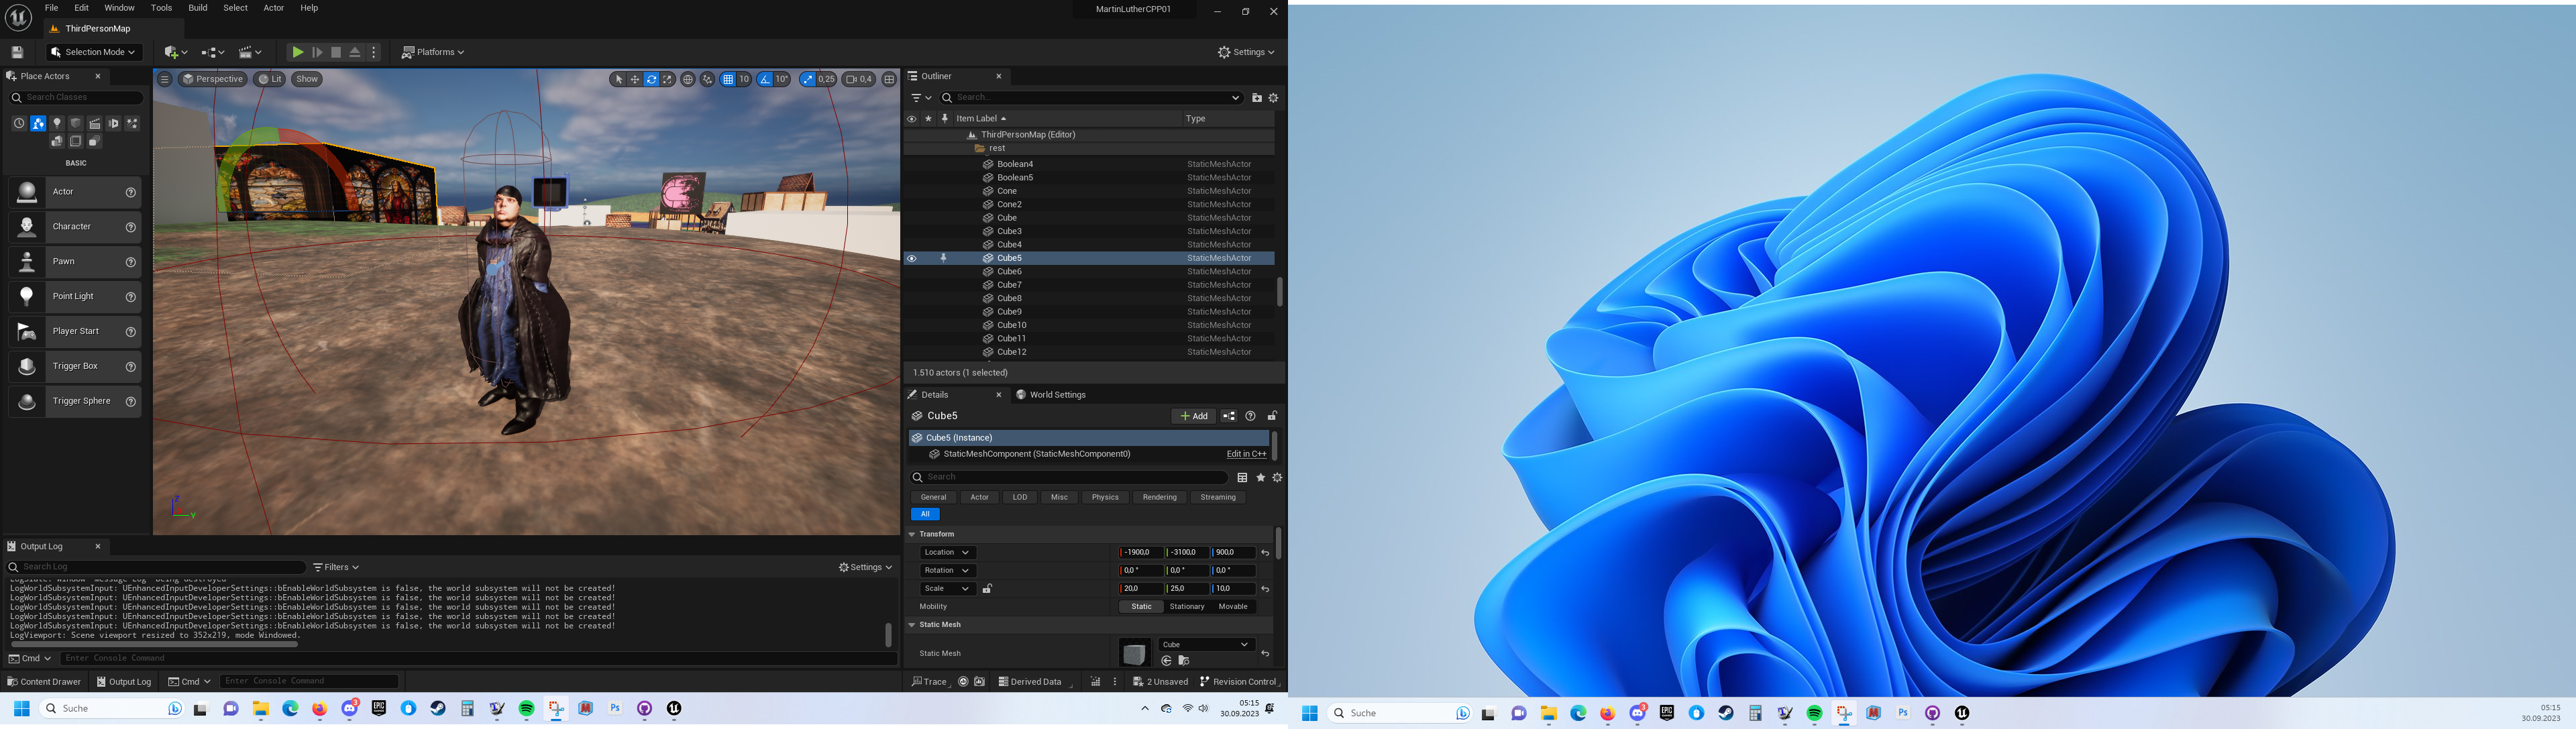
\includegraphics[width=14cm]{BilderFuerBA/Screenshot/MartinLutherImSpiel.png}
	\caption{UE5: Martin Luther im Spiel}
	\label{MartinLutherImSpiel}
\end{figure}

\begin{figure}
	\centering
	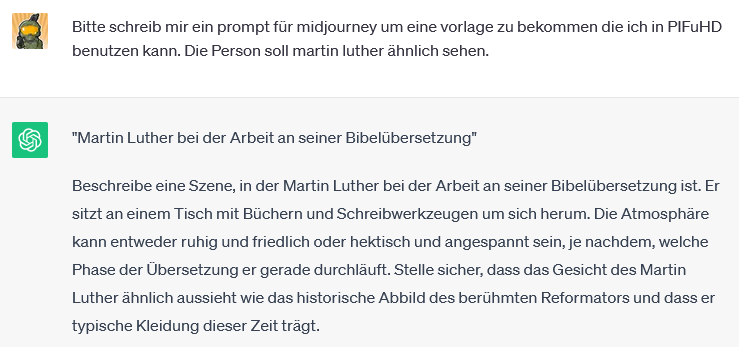
\includegraphics[width=14cm]{BilderFuerBA/CGPTMidJourneyMartinLuther/02.png}
	\caption{ChatGPT: Erster Versuch zur erstellung eines Promt für Midjourney}
	\label{ChatGPT_erster_Versuch_Midjourney_Promt}
\end{figure}

\begin{figure}
	\centering
	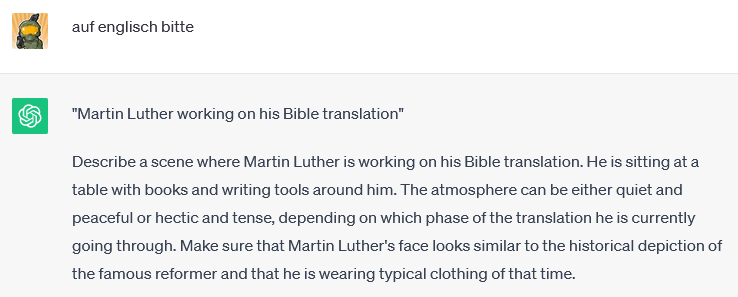
\includegraphics[width=14cm]{BilderFuerBA/CGPTMidJourneyMartinLuther/03.png}
	\caption{ChatGPT: Übersetzung des Prompts}
	\label{ChatGPT_übersetzen}
\end{figure}

\begin{figure}
	\centering
	\begin{minipage}[t]{0.45\linewidth}
		\centering
		\includegraphics[width=6.405cm]{BilderFuerBA/MJ/Busfahrer.png}
		\caption{Midjourney Prompt: Bussfahrer}
		\label{Bussfahrer}
	\end{minipage}
	\hfill
	\begin{minipage}[t]{0.45\linewidth}
		\centering
		\includegraphics[width=6.405cm]{BilderFuerBA/MJ/bus_driver.png}
		\caption{Midjourney Prompt: bus driver}
		\label{bus_driver}
	\end{minipage}
\end{figure}



\begin{figure}
    \centering
    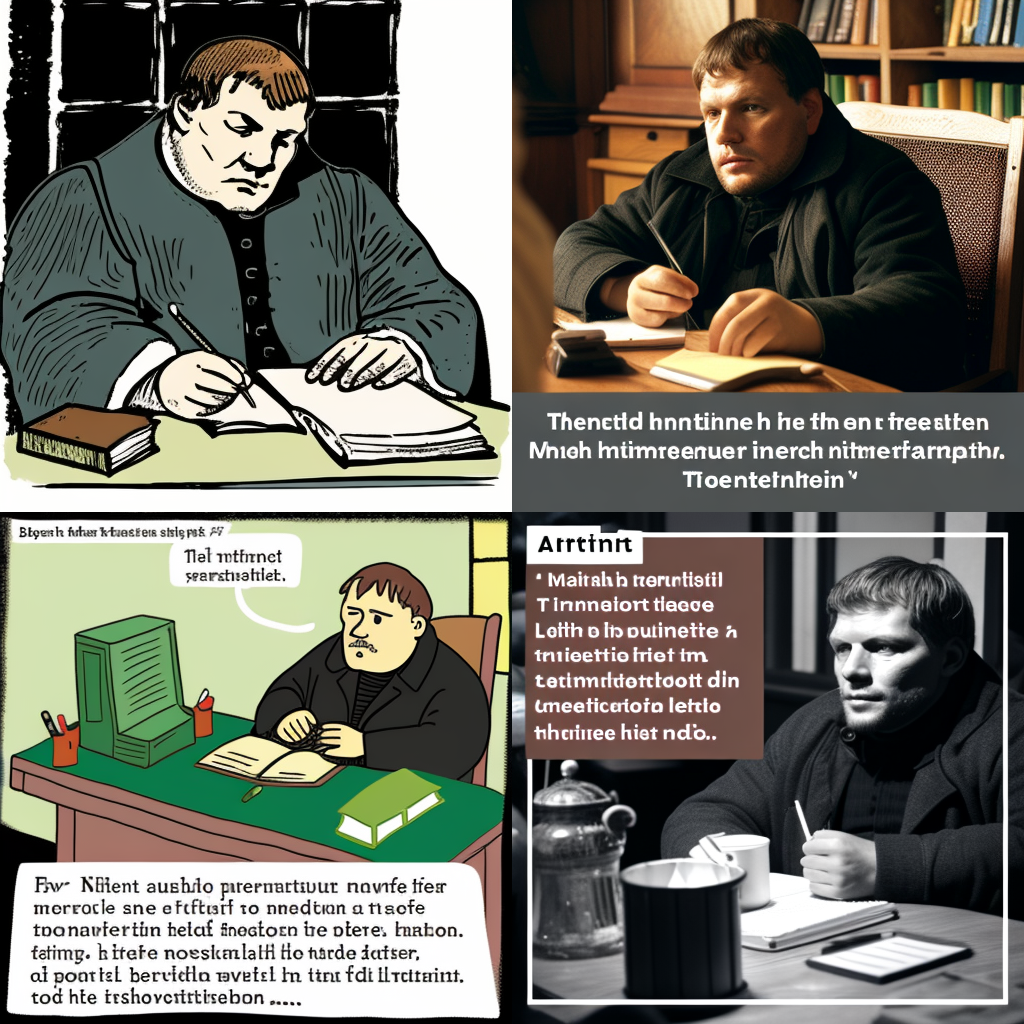
\includegraphics[width=8.022cm]{BilderFuerBA/MJ/MLaufEnglisch.png}
    \caption{Midjourney: Erster Prompt von ChatCPT}
    \label{Midjourney_erster_Prompt}
\end{figure}

\begin{figure}
    \centering
    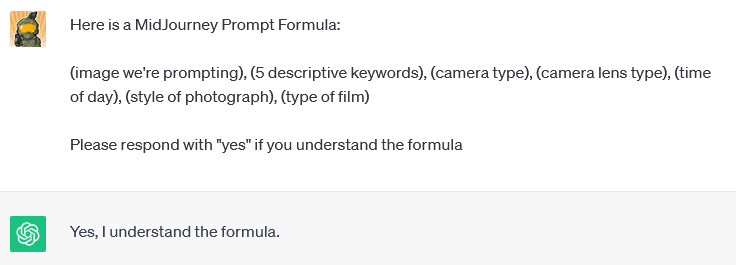
\includegraphics[width=14cm]{BilderFuerBA/CGPTMidJourneyMartinLuther/04.png}
    \caption{ChatGPT: Aufforderung verwendung einer Midjourney-Formel}
    \label{chatgpt-ptompt-Midjourney-04}
\end{figure}
\begin{figure}
    \centering
    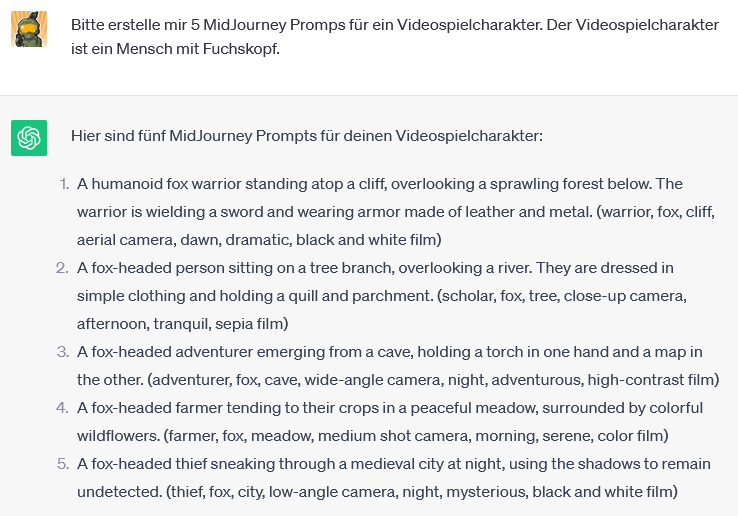
\includegraphics[width=14cm]{BilderFuerBA/CGPTMidJourneyMartinLuther/05.png}
    \caption{ChatGPT: Erstellung Prompts mit Verwendung der Midjourney-Formel}
    \label{chatgpt_mj-formel_mit_Klammern}
\end{figure}

\begin{figure}
	\centering
	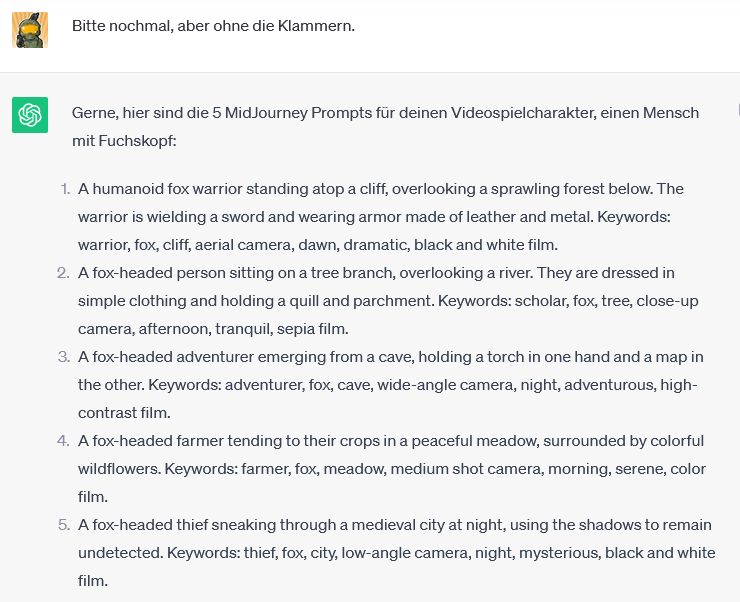
\includegraphics[scale=0.7]{BilderFuerBA/CGPTMidJourneyMartinLuther/06.png}
	\caption{ChatGPT: ChatGPT erstellt Promt für Midjourney in Englisch und ohne Klammern}
	\label{chatgpt_mj-formel_ohne_Klammern}
\end{figure}

\begin{figure}
	\centering
	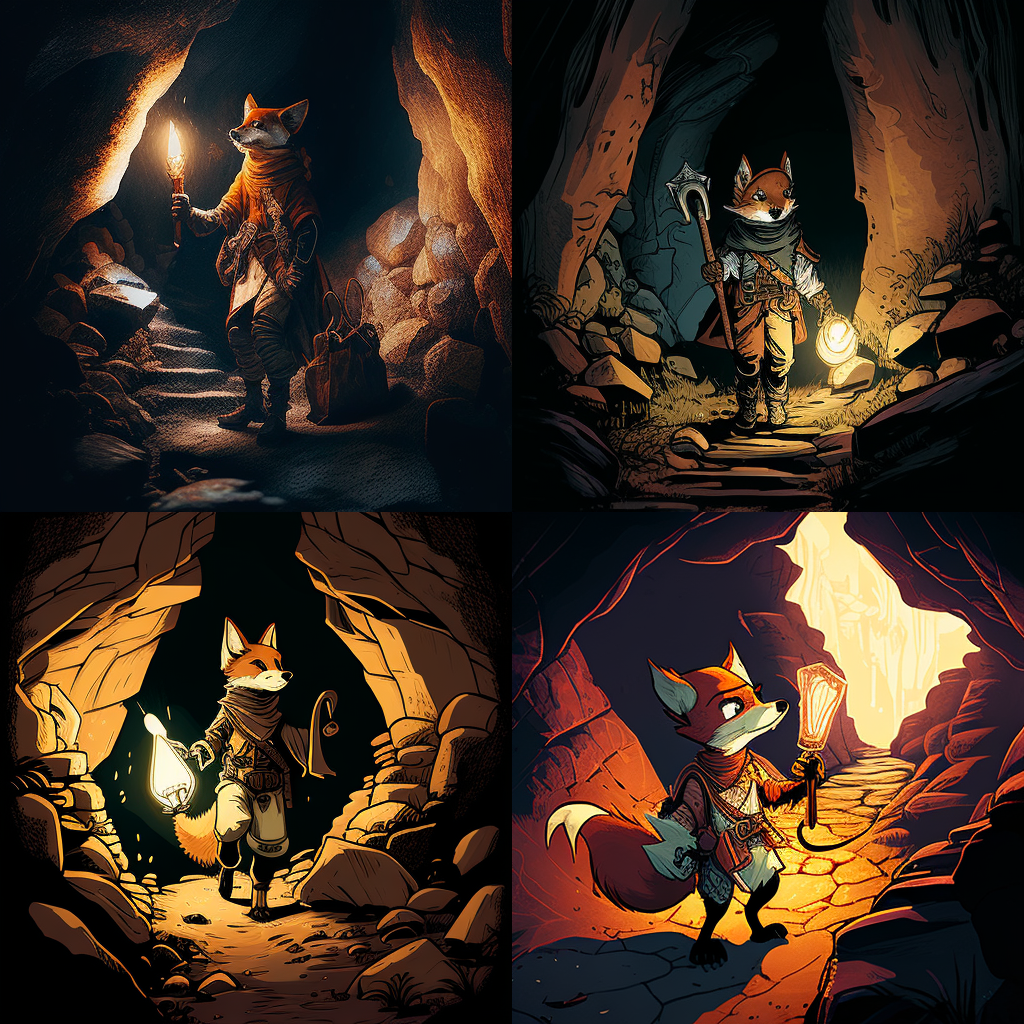
\includegraphics[width=8.022cm]{BilderFuerBA/Sonstiges/fuchsKopfAbenteuerer.png}
	\caption{Midjourney: Promt eines Abenteurers mit einem Fuchskopf}
	\label{MidjourneyFuchsKopfAbenteuerer}
\end{figure}

\begin{figure}
	\centering
	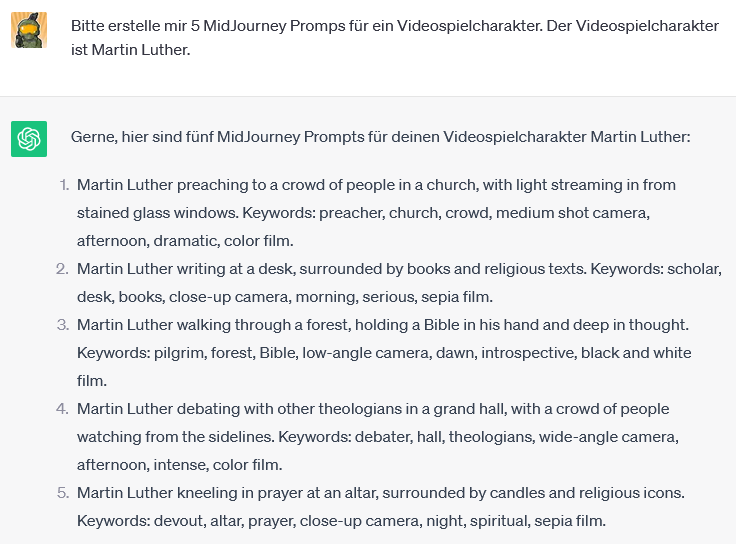
\includegraphics[scale=0.7]{BilderFuerBA/CGPTMidJourneyMartinLuther/07.png}
	\caption{ChatGPT: Midjourney Prompt für Martin Luther als Spielfigur}
	\label{chatgptMartinLutherMJformelErstenFünf}
\end{figure}


\begin{figure}
	\centering
	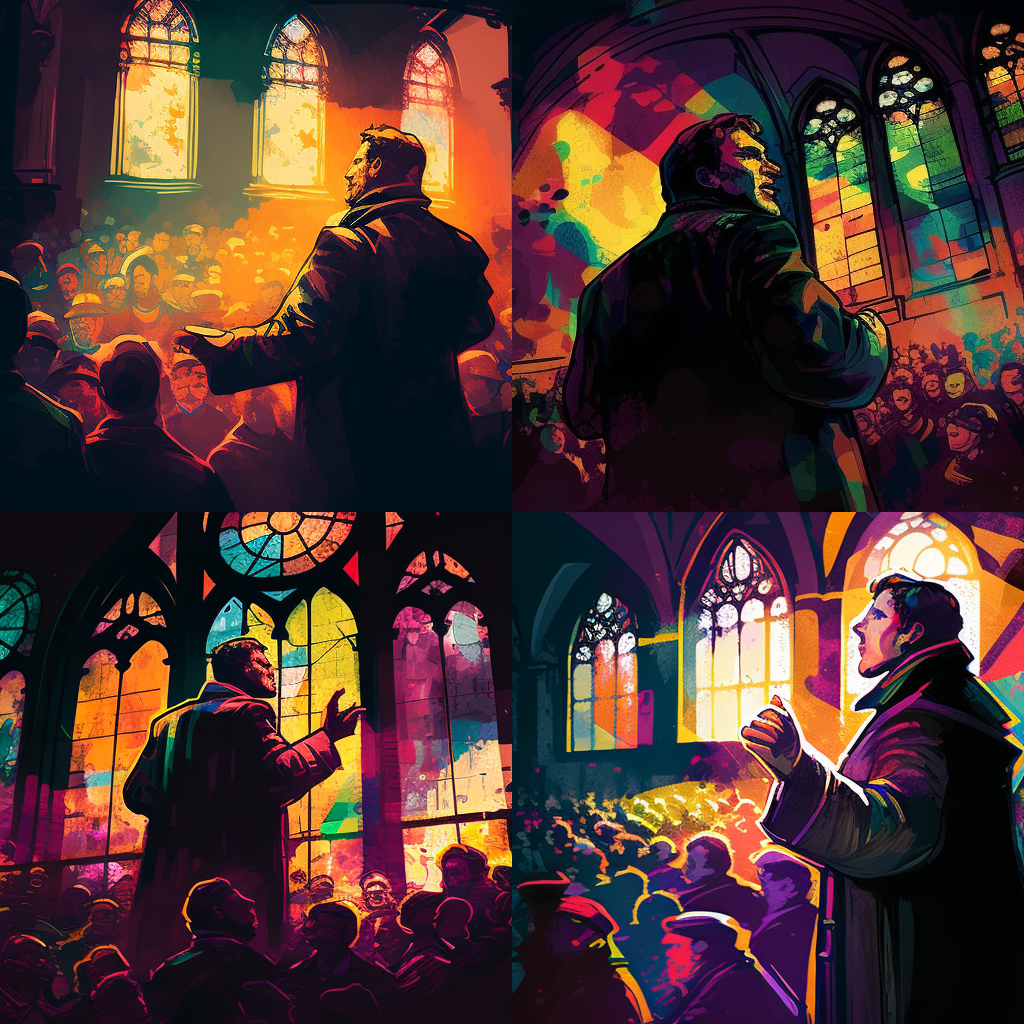
\includegraphics[width=8.022cm]{BilderFuerBA/MJ/MidJourneyMLMitFormel.png}
	\caption{Midjourney: Martin Luther Promt mit Midjourney-Formel}
	\label{MidJourneyMLMitFormel}
\end{figure}

\begin{figure}
	\centering
	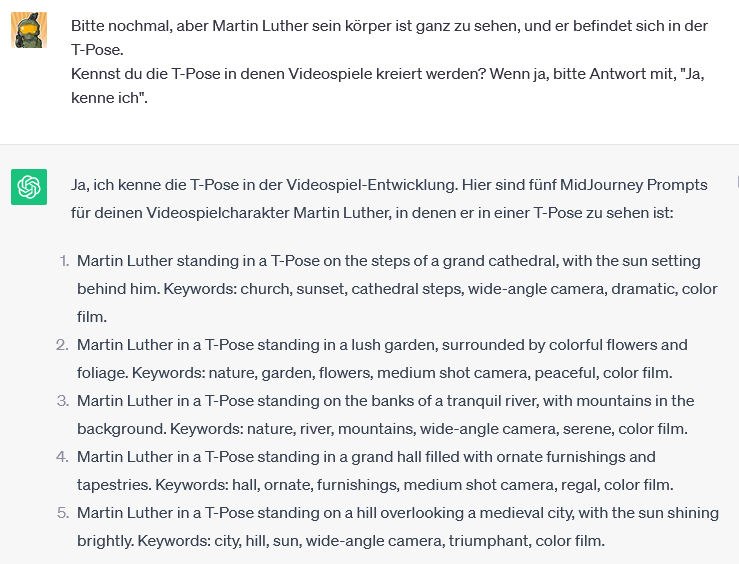
\includegraphics[scale=0.7]{BilderFuerBA/CGPTMidJourneyMartinLuther/09.png}
	\caption{ChatGPT: Midjourney Prompt für Martin Luther in T-Pose}
	\label{chatgptMartinLutherMJinTPose}
\end{figure}

\begin{figure}
	\centering
	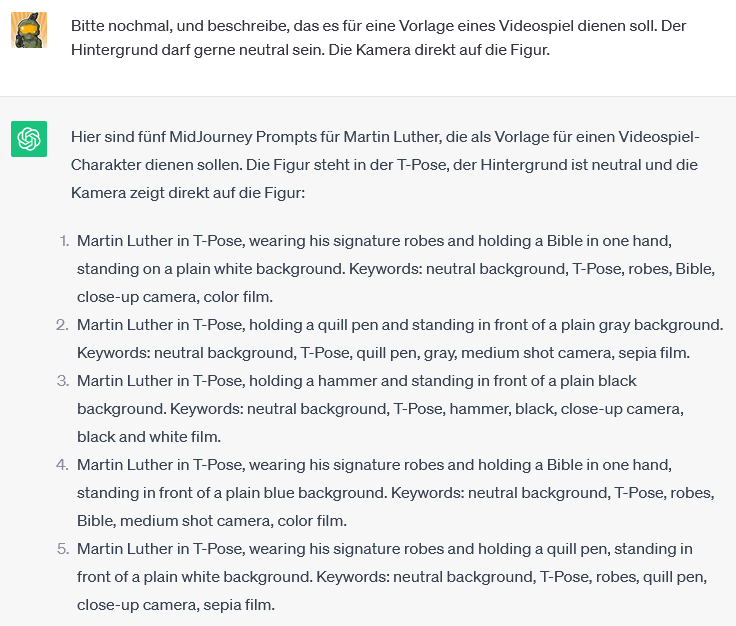
\includegraphics[scale=0.7]{BilderFuerBA/CGPTMidJourneyMartinLuther/10.png}
	\caption{ChatGPT: Midjourney Prompt für Martin Luther in T-Pose}
	\label{chatgptMartinLutherMJmitNeutralenHintergrund}
\end{figure}

\begin{figure}
	\centering
	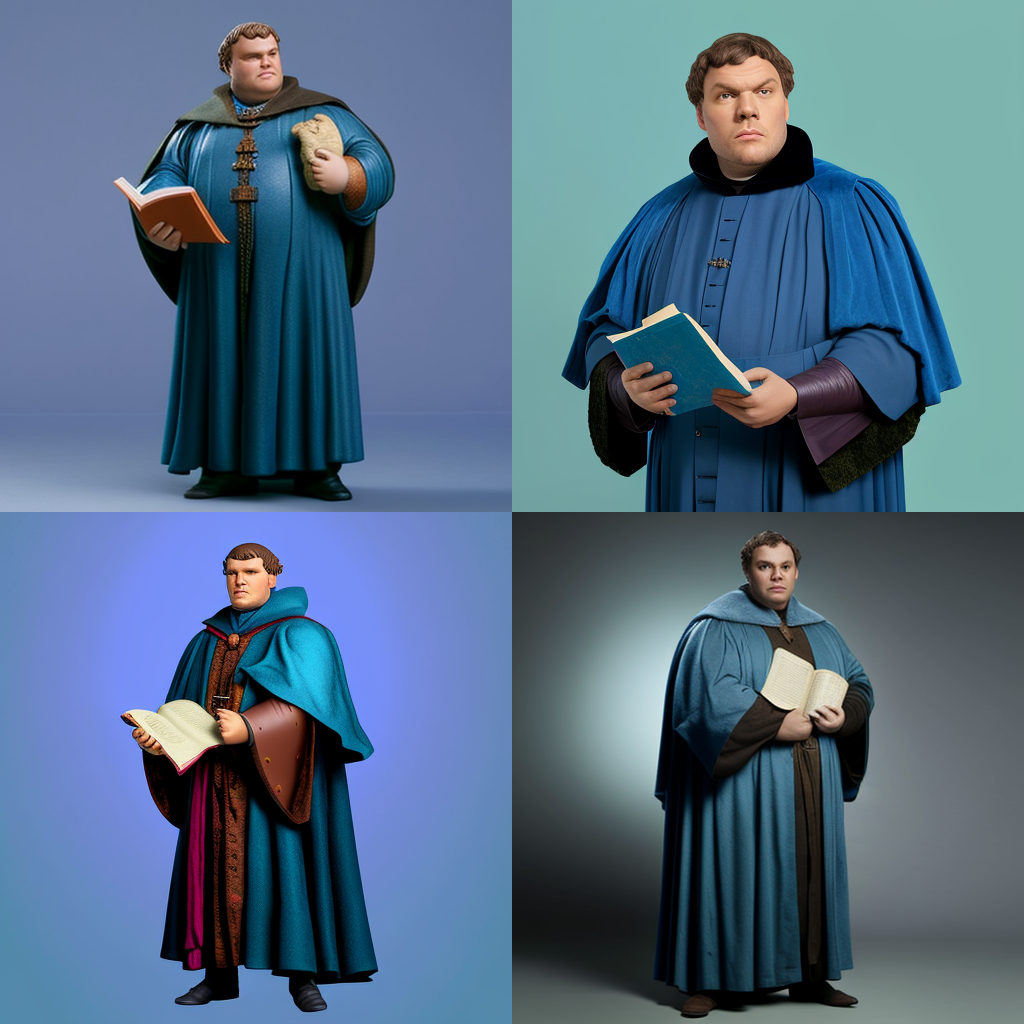
\includegraphics[width=8.022cm]{BilderFuerBA/MJ/MartinLutherInTPoseFirst.png}
	\caption{Midjourney: Martin Luther Promt versuch in T-Pose, neutralen Hintergrund und direkte Kamera}
	\label{MartinLutherInTPoseNeutralerHintergrundDirekteKamera}
\end{figure}

\begin{figure}
	\centering
	\includegraphics[width=8.022cm]{BilderFuerBA/MJ/ErsteAusgabeVomFinalenPrompt.png}
	\caption{Midjourney: Erste Ausgabe vom finalen Prompt}
	\label{ErsteAusgabeVomFinalenPrompt}
\end{figure}

\begin{figure}
	\centering
	\includegraphics[width=8.022cm]{BilderFuerBA/MJ/ZweiteAusgabeVomFinalenPrompt.png}
	\caption{Midjourney: Vier weitere Variation von Version Zwei}
	\label{ZweiteAusgabeVomFinalenPrompt}
\end{figure}

\begin{figure}
	\centering
	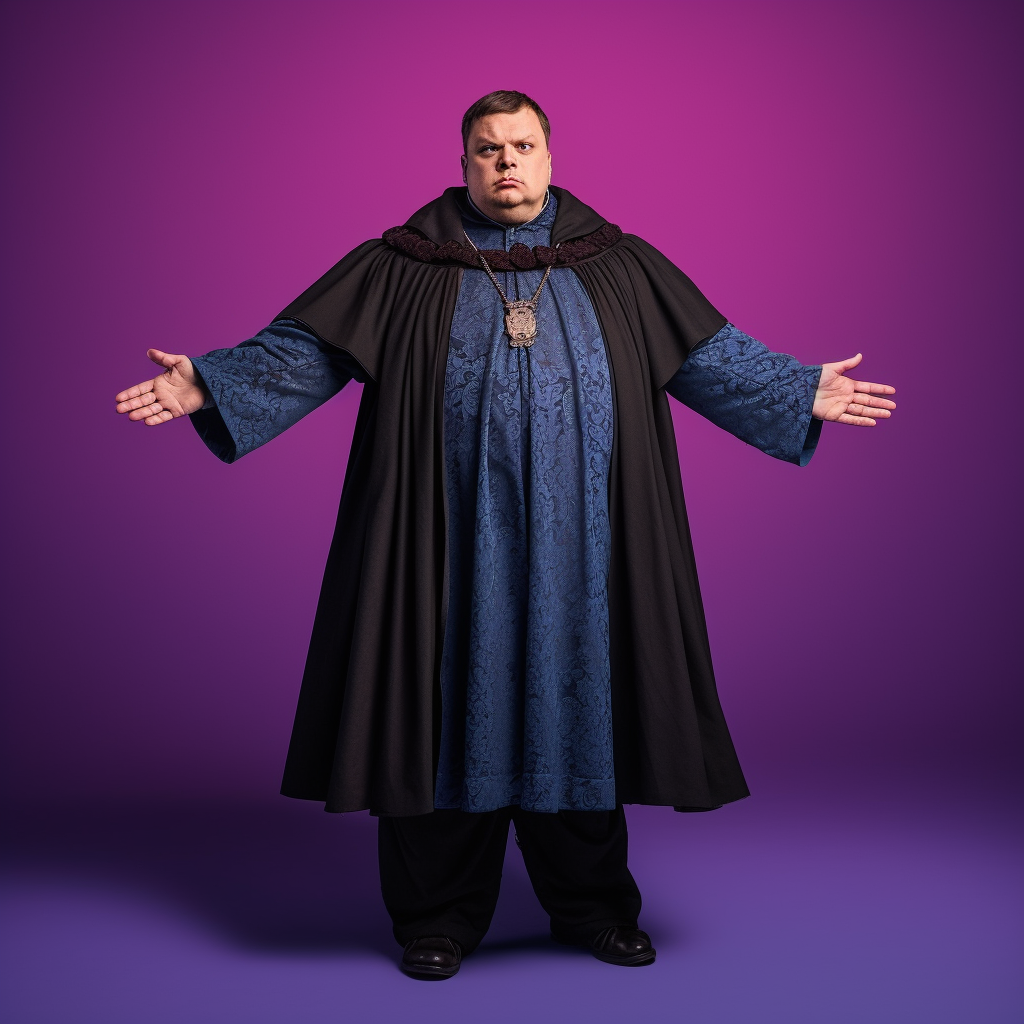
\includegraphics[width=8.022cm]{BilderFuerBA/MJ/DritteAusgabeVomFinalenPrompt.png}
	\caption{Midjourney: Hochskaliertes Endresultat von Version Vier}
	\label{DritteAusgabeVomFinalenPrompt}
\end{figure}

Auf Abbildung \ref{MartinLutherImSpiel} ist die Huptspielfigur des Prototypes zu Sehen. Die Hauptfigur ist Martin Luther nachempfunden. Die Hauptspielfigur ist vom Spieler Steuerbar und wurde mit Hilfe den KI-Systemen ChatGPT, Midjourney und PIFuHD erstellt. Wie die soben genannten KI-Systeme verwendet wurden, werde ich in den folgenden Absätzen ausfühlich erklären
\\
Ich beginne die Entwicklung der Hauptfigur in dem ich ChatGPT um eine Beschreibung meiner Hauptfigur auffordere. Ich gebe ebenfalls an, dass ich die Ausgabe von ChatGPT als Prompt für Midjourney verwenden möchte. Zusätzlich fordere ich ChatGPT auf, dass das Ergebnis von Midjourney für PIFuHD kompatibel sein soll.
\\
Mit der in Abbildung \ref{ChatGPT_erster_Versuch_Midjourney_Promt} zusehenden Aufforderung, habe ich eine deutsche Ausgabe bekommen. Durch eine weitere kurze Aufforderung wie in Abbildung \ref{ChatGPT_übersetzen} wurde die Ausgabe von ChatGPT übersetzt.
\\
Midjourney liefert in Englisch in Gegensatz im Vergleich zu Deutsch oft unterschiedliche Ergebnisse. Beobachten kann das zum Beispiel in Abbildung \ref{Bussfahrer} Bussfahrer auf deutsch, und in Abbildung \ref{bus_driver} buss driver auf englisch.
\\
Anhang in Abbildung \ref{Bussfahrer} und Abbildung \ref{bus_driver} kann man gut beobachten, dass die verwendeten Sprache ein Unterschied macht. Im Englischen wird eher eine Person dargestellt, die ein Lenkrad in der Hand hält, wo der Prompt auf deutsch eher ein Passagier dargestellt wird oder ein Bus in einer Landschaft.
\\
%https://philipp-stelzel.com/de/midjourney-deutsch-sprachen/ Abrufdatum 25.09.2023
Midjourney versteht nicht unsere Sprache, sondert die Genauigkeit entsteht aus der Menge der Daten womit das KI-System Trainiert ist. Das Wort Bussfahrer kommt womöglich mit nicht so oft in den Trainigsdaten vor wie buss driver aus dem Englischen.
\\
Mit dieser Erkenntnis, entscheide ich mich meine Promts auf Englisch für Midjourney zu verfassen bzw von ChatGPT verfassen lassen.
\\
Nach der Übersetzung von ChatGPT, übergebe ich den von ChatGPT generierten Promt Midjourney. Das Ergebnis is in Abbildung \ref{Midjourney_erster_Prompt} zu betrachen.
\\
In Abbildung \ref{Midjourney_erster_Prompt} ist zu sehen, das Midjourney immer Vier bilder als Vorschau ausgibt. Midjourney bietet über sein User-Interface drei Möglichkeiten um mit dem Ergebnis weiter zu Arbeiten.
\begin{itemize}
	\item 1 Vier weitere Versionen auf grundlage von Version 1 bis 4
	\item 2 Eine Hochskallierte Version von 1 bis 4
	\item 3 Vier neue weitere Versionen
\end{itemize}
Oben links befindet sich Version 1, oben rechts Version 2, unten links Version 3 und unten rechts Verion 4.
\\
Der Prompt von ChatGPT aus Abbildung \ref{ChatGPT_übersetzen} beinhaltet sehr viele Schlüsselwörter die in Textform verfasst sind. Ich beschreibe den Promt von ChatGPT sehr Athomsphärisch, wie als würde man eine Textstelle aus einem Roman lesen, anstelle einer Aufforderung gegenüber eines KI-System.
\\
Ich vermutet, dass ChatGPT nicht genügend darauf trainiert ist, wie Midjourney-Prompts auszusehen haben.
\\
Eine Recherche auf YouTube hat gezeigt, dass das Verwenden von Midjourney-Formeln ein aufgeräumtes Ergebnis hervorbringen kann. Eine Kurze Auforderung wie in Abbildung \ref{chatgpt_formel_mj_first_5} kann bessere Ergebnisse bei Midjourney gewähren.
\\
Im ersten Test werden die Prompts mit Klammern \ref{chatgpt_mj-formel_mit_Klammern} ausgegeben. Diese sind mit einer einfachen Aufforderung wie in \ref{chatgpt_mj-formel_ohne_Klammern} möglich zu entfernen.
\\
Ich habe die Ausgabe mit dem Fuchskopf Midjourney übergeben und das ergebnis ist in Abbildung \ref{MidjourneyFuchsKopfAbenteuerer} zu sehen.
\\
Mit den Ergebnissen bin ich so weit zufrieden, da mein Hauptcharakter kein Abenteuerer mit Fuchskopf ist, sonder Martin Luther nachempfunden sein soll, habe ich ChatGPT dazu Aufgefordert mir 5 Promts für Midjourney zu erstellen. Die ergebnisse von ChatGPT ist in Abbildung \ref{chatgptMartinLutherMJformelErstenFünf} zu sehen. Die dazu entsandenen Bilder von Midjourney sind in Abbildung \ref{MidJourneyMLMitFormel} zu sehen.
\\
Der Vorteil dieser Methode ist, das man nun einzelne Parameter in der Midjourney-Formel belieben verändern kann um ein Gewünschtes Ergebnis zu erlangen. Das Ziel ist es ein "Foto" von Martin Luther zu bekommen um es später für PIFuHD zu verwenden. Das Ergebnis von Abbildung \ref{MidJourneyMLMitFormel} ist noch nicht zu verwenden, da zu viele Fabenfrohe Deteils zu sehen sind. PIFuHD weist darauf hin das Bilder am besten funktionieren wenn:
\begin{itemize}
	\item Bilder eine Mindestauflösung von 512 x 512 Pixel haben.
	\item Bilder wo nur eine Person abgebildet sind.
	\item Bilder wo die Person direkt in die Kamera schauen.
	\item Bilder wo die Person gut beleuchtet ist.
	\item Bilder wo die Person vor einem Einfachen Hintergund stehen.
\end{itemize}

Um diese Punkte zu beachten habe ich folgende Parameter von ChatGPT überarbeiten lassen. Als erstes soll der Charakter in der T-Poste stellung sein Abbildung \ref{chatgptMartinLutherMJinTPose} anschließend mit einem Neutralen Hintergrund und einer direkten Kamere auf die Figur. Das Ergebnis ist in Abbildung \ref{MartinLutherInTPoseNeutralerHintergrundDirekteKamera} zu sehen.
\\
An dieser Stelle habe ich nicht mehr mit ChatGPT für die Hauptfigur gearbeitet. Ab hier habe ich sehr viel ausprobiert um eine Fotoähnliche abbildung von Martin Luther zu bekommen. Der Finale Prompt der am ende das Bild von Martin Luther generiert hat war:
\\
the famous martin luther from germany, robe from the Renaissance, T-Pose for gamedesign, standing in front of a plain blue background. neutral magenta background, T-Pose, whole body, face looking in the camera, color film
\\
Midjourney
Mit diesem Prompt habe ich es geschafft mit Version 2 in Abbildung \ref{ErsteAusgabeVomFinalenPrompt} ein Ergebnis zu generieren was meine Anforderung als Game Designer entprechen. Ich habe ein, gerade in die Kamera schauende Mann der Martin Luther ähnlich sieht. Der Mann steht in einer T-Pose. Der Hintergrund ist farbarm / neutral und wir sehen den kompletten Körper.
\\
Durch die betätigung des Buttons V2 bekomme ich 4 weiter Versionen auf grundlage von Version 2 aus der Abbildung \ref{ErsteAusgabeVomFinalenPrompt}.
\\
Abbildung \ref{ZweiteAusgabeVomFinalenPrompt} zeigt vier weitere Versionen von Version 2 der Ausgabe \ref{ErsteAusgabeVomFinalenPrompt}. Die Unterschiede sind viel geringer und unterscheiden sich in diesem Beispiel am größten an der Frisur, den Oberteil der Robe und der Kette. Den rest empfinde ich sehr ähnlich.
\\
Besonder die Kette ist ein Deteil was mich als Game Designer am meisten angesprochen hat, was mich am Ende dazu entschieden hat, Version Vier über den Button U4 hochzuskaliern.
\\
Die hochskalierte Version von Abbildung \ref{ZweiteAusgabeVomFinalenPrompt} ist in Abbildung \ref{DritteAusgabeVomFinalenPrompt} zu betrachten.
\\
Wir sehen einen Mann in einer Kirchlich anmutenen Robe. Sein Haar ist braun, seine Haut hell. Der Mann trägt beide Arme vom Körper so das die Handinnenfläche zur Kamera zeigen.
\\
Dieses Bild verwende ich um ein 3D-Modell von Martin Luther zu verwenden.
\subsubsection{Erzeugen eines 3D-Modells mit Hilfe von PIFuHD}
\begin{figure}
	\centering
	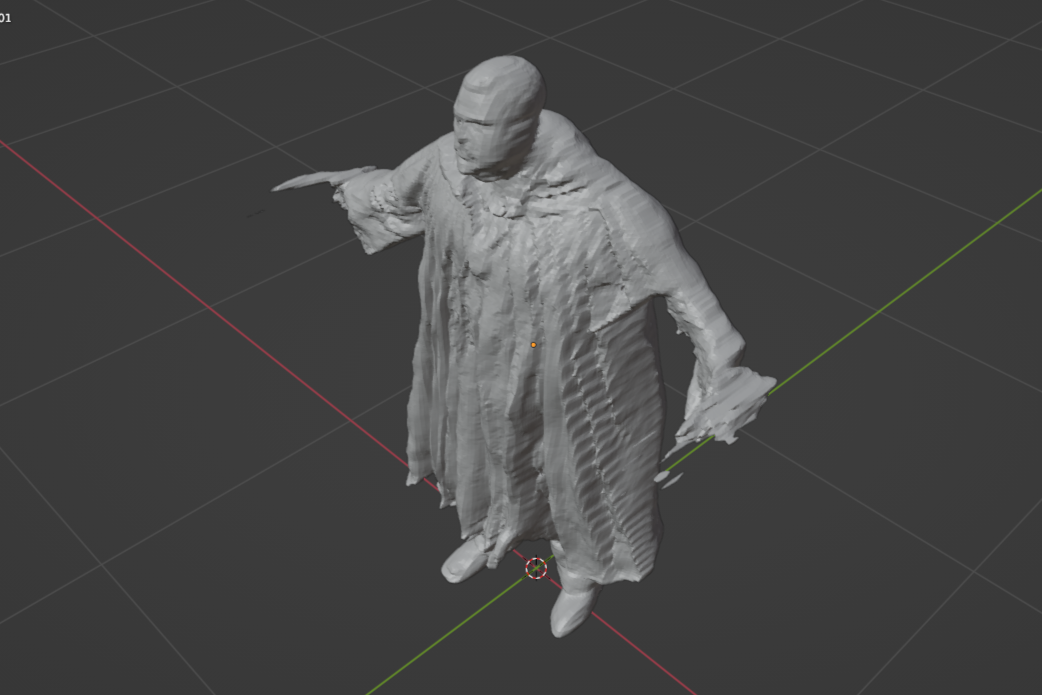
\includegraphics[width=14cm]{BilderFuerBA/Screenshot/BlenderMLVonPIFuHD105k.png}
	\caption{Blender: 3D-Modell von Martin Luther von PIFuHD}
	\label{BlenderMLVonPIFuHD105k}
\end{figure}
\begin{figure}
	\centering
	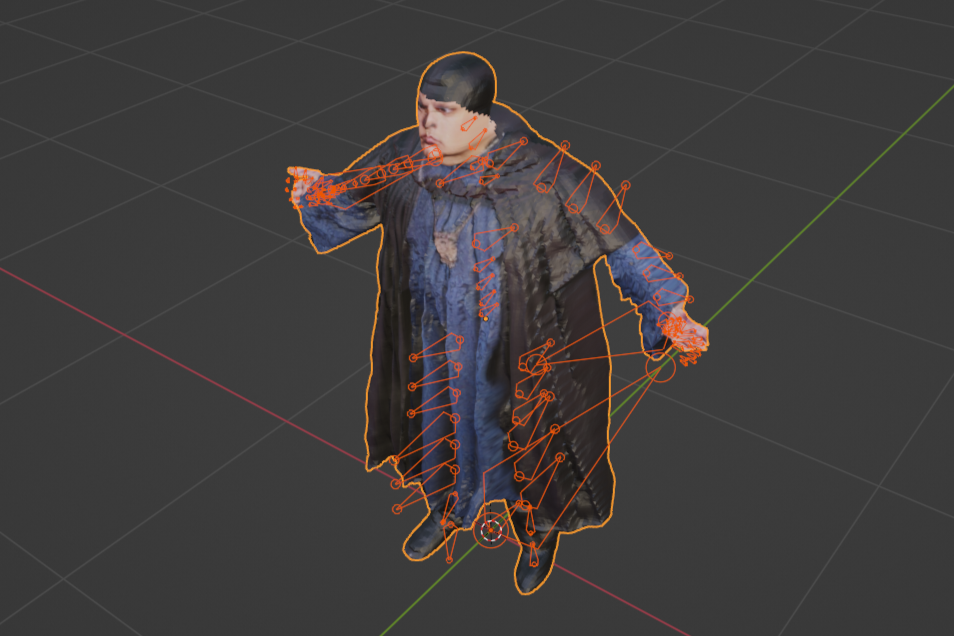
\includegraphics[width=14cm]{BilderFuerBA/Screenshot/BlenderMLGeriggtUndTexturiert95k.png}
	\caption{Blender: Martin Luther Texturiert, geriggt, Nachgebessert und gemergeten Verticies}
	\label{BlenderMLVonPIFuHD105k}
\end{figure}
In Abbildung \ref{BlenderMLVonPIFuHD105k} zeigt das 3D-Modell von Martin Luther welches durch das KI-System PIFuHD erzeugt ist.
\\
PIFuHD ist durch eine Google-Suche zu finden. Der Erste Vorschlag von Google zeigt eine Git-Hub-Link an. Im kopf dieser Git-Hub Seite findet man weit oben den Link mit der Bezeichnung Demo.
\\
Ich habe die Demo über Google-Colab zum laufen bekommen in dem ich mich über mein Google-Konto anmelde und auf Verbinden mit gehosteter Laufzeit: GPU klicke.
\\
Anschließend kann über den Menüpunkt Laufzeit -> Alle ausführen oder alternativ CTRL + F9 PIFuHD ausführen.
\\
Weiter unten in der Website befindet sich der Abschnitt Config input data. An dieser Stelle wartet PIFuHD auf eine Eingabeauforderung, wo ich mein Bild von Abbildung \ref{DritteAusgabeVomFinalenPrompt} übergebe.
\\
Die Übergabe folgt über den Button Durchsuchen.... Ist die Übergabe erfolgreich, erfolgt die Ausgabe über der Ordnerstruktur links.
\\
Meine obj-Datei befindet sich unter pifuhd -> results -> pifuhd-final -> recon. Zusätlich zu meiner obj-Datei bietet PIFuHD mir eine png-Datei an, was eine Normalmap darstell und eine mp4-datei die ein fünf sekündiges Video von meinem 3D-Modell zeigt.
\\

%todo Polycount, UVs und narnite erklären verionsnummern hinzufügen
\subsubsection{Polycount verringern in Blender}
in Blender kann über den Menüpunkt File -> Import -> Wavefront die Obj-Datei importiert werden. 
\\
Das verringern des Polycount bewirkt, dass im späteren Prototyp weniger rechenkapazität verwendet wird. Besonder bei der Spielfigur ist es wichtig, da die Unreal Egine 5 aktuell Narnite nur für unbeweglich Objekte in der Spielwelt verfügbar macht.
Nachdem ich die Obj-Datei in Blender Importiert habe, wechsel ich in den Eddit.
\\
Im Edit Mode wähle ich ein Verticie aus. Mit STRG + L wähle ich alle mit dem Modell verbundene Verticies aus. Das Modell erscheint nun Orange.
\\
Mit der Tastenkombination STRG + I invertiere ich die Auswahl. Nun habe ich alle Verticies ausgewählt die nicht direkt Mit dem 3D-Modell verbunden sind.
\\
Mit der der Taste ENTF ist es mir nun möglich alle Verticies zu löschen die auserhalb des 3D-Modells liegen
\\
Nachdem alle Verticies auserhalb des 3D-Modells gelöscht sind wähle ich alle Verticies aus in dem ich die A-Taste einmal drücke.
\\
Nun sind alle Verticies vollständig ausgewählt.
\\
Mit dem Shortcut M ist es mir nun möglich das 3D-Modell zu mergen.
\\
Ich Merge mein 3D-Modell mit der Funktion By Distance.
\\
Unten links öffnet sich ein kleines Untermenü mit dem Namen Merge by Distance und verbessere den wert auf 0,001 m.
\\
Durch dieses Verfahren habe ich den Polywert von knapp 120.000 Verticies auf 98.000 Verticies verringert, was eine Verringerung von rund 18\% ist.
\subsubsection{Artefakte bereinigen in Blender}
Blender gibt eine vielzahl an Möglichkeiten sein 3D-Modell zu moddelieren. Ich habe nachdem ich den Polycount reduziert habe betreffende Stellen im Edit Mode makiert und gemerget. Ein weiteres Verfahren war im Sculp Mode die verschiedenen Sculpwerkzeuge zu verwenden wie zum Beispiel Draw.
\subsubsection{Texturieren in Blender}
zweites bearbeitungsfenster hinzufügen auf UV-Editor umstellen über menüpunkt Image - Open das gewünschte foto... die kamera so einstellen das es ungefähr die gleiche blickrichtung auf das model hat wie im bild... in dem beispiel kann man über das numbap 1 für frontalansich wählen..
im modell alles makieren und mit dem shortkut u für unwrap die funktion Projekt from View auswählen.
Skallieren im UV Editor
Ich habe das 3D-Modell mit Hilfe der von Midjourne erzeugten Bildes in Blender Texturiert.
\\
Blender bietet mir die Möglichkeit ein zweites Bearbeitungsfenster hinzuzufügen, welche ist dann als UV Editor benutze.
\\
Über den Menüpunkt Image -> Open, füge ich Abbildung: \ref{DritteAusgabeVomFinalenPrompt} ein, um UVs des 3D-Modells zu editieren.
\\
Rechts über das Propertie-Fenster -> Material Properties -> auf dem gelben Punkt neben Base Color -> Image Textur habe ich nun die Möglichkeit, ebenfalls Das Bild aus Abbildung \ref{DritteAusgabeVomFinalenPrompt} zu wählen.
\\
Damit das Bild von Martin Luther korrekt auf das 3D-Modell von Martin Luther korrekt projeziert wird, wähle ich eine Kamera einstellung, das ungefähr die Kameraeinstellung entsprich, wie das Bild von Martin Luther.
\\
Durch die betätigung der 1 auf meinem Numpad wird die Kamera so eingestellt das ich eine frontale ansicht meines 3D-Modells im Edit Modus habe.
\\
Ich Makiere alle Verticies in dem ich den Shortcut A drücke. Anschließend Unwrape ich mein 3D-Modell in dem ich den Shortcut U drücke.
\\
Blender bietet mir verschiedene Fuktionen an, mein 3D-Modell zu Unwrapen. Ich wähle die Fuktion Project from View.
\\
In meinem UV-Editor habe ich nun die Möglichkeit, das Projezierte 3D-Modell so zu skalieren das es mit der Vorlage übereinstimmt.
\\
Das Problem nach dem Unwrapen nach dieser beschriebenen Methode ist, dass das 3D-Modell von Vorne genauso texturiert ist wie von Hinten.
\\
Um den Rücken und den Hinterkopf einigermaßen korrekt zu texturieren, wähle ich in meinem gewünschten bereichen des 3D-Modells die ensprechenden bereiche aus und verschiebe sie im UV-Editor in gegenden, die zu dieser Stelle passen würde.
\\
Zum Beispiel der Mittelteil der Robe, der blau gefärbt ist, verschiebe ich in eine etwas brauneren Region im UV-Editor.
\\
Nachdem ich den Rücken und den Kopf nachtexturiert habe, fehlt noch ein letzer wichtiger schritt, damit Martin Luther in der Unreal Engine zum Leben erweckt wird, und zwar das Rigging.
\subsubsection{Rigging in Blender}%todo rigging erklären
Damit mein Hauptcharakter nicht nur in seiner T-Pose verweilt wenn er läuft und Springt, sonder Arme Beine und Kopf bewegt, braucht das 3D-Modell von Martin Luther ein Skeleton-Mesh.
\\
Damit ich ein 3D-Modell für die Unreal Engine 5 riggen kann, benötige ich das Blander Addon Game Rig Tools von CGDive.
\\
Über den Button Initiate Mannequin fügt das Addon ein Unreal Engine 5 kompatibles Skeleton Mesh zu unserem 3D-Modell.
\\
Über das UE5\_Manny\_TWEAK das ich über die Scene Collection ausweghelen kann, bewege ich die einzelnen Bones des Skeleton mesh innerhalb des 3D-Modells. Mit dem Shortcut G kann ich im Pose Mode die einzelnen Bones bewegen. von Martin Luther so plazieren wie bei einem normalen Menschen auch.
\\
Nachdem ich die Bones vom UE5\_Manny\_TWEAK fertig plaziert habe, kann ich über das Addon-Fenster von Game Rig Tool, Unreal-Rig nur sichtbar machen in den ich auf den Weißen Punkt neben Unreal drücke. 
\\
Nachdem nur noch unser 3D-Modell und das Unreal-Rig sichtbar ist wächsel ich in den Object Mode und wähle erst mein 3D-Modell aus und mit Schift-Taste gedrückt das Unreal-Rig aus.
\\
Über den Menüpunkt File -> Export -> FBX kann ich über das gerigte Modell speichern. Beim Speichern wähle ich folgende Optionen aus:
\begin{itemize}
	\item Limit to Selected Objects 
	\item Object Types Amature und Mesh
	\item Unter Transform bestätige ich noch das Apply Transform
	\item Unter Geometry wähle ich unter Smoothing Face
	\item Unter Armature stelle ich Add Leaf Bones aus
	\item Unter Bake Animation stelle ich ebenfalls aus
\end{itemize}
Nachdem ich diese Einstellung getätigt habe, wähle ich noch ein Namen aus für meine FBX-Datei und drücke auf Export FBX.
%
%
%
%
%
%
%
Mit diesen Einstellungen kann ich das 3D-Modell Unwrapen. Über das Shortcut U -> Project from View werden die UV-Informationen neu definiert.
\\
Da ich eine sehr direkte Kamera einstellung auf meiner vorlage in \ref{DritteAusgabeVomFinalenPrompt} habe, brauche ich nur die Taste 1 auf meinem NumPad der Tastatatur drücken um eine direkte ansich auf mein §D-Modell zu bekommen in meinem Bearbeitungsfenster wo ich den Edit Mode geöffnet habe.

\ref{chatgptMartinLutherMJmitNeutralenHintergrund} was sehr viele Probleme verurschat hat. Midjourney versteht den begrif T-Pose nicht und 
\\
Mein ziel ist es Bilder von Midjourney zu erhalten, die wie Fostos von Personen wirken. Mit diesen Fotos dienen dazu mit PIFuHD zu übergebn um 3D-Modelle von einer Person zu bekommen.
\\
Dieses Modell möchte ich in meinem Prototyp verwenden um eine Spielfigur zu erzeugen.
\\
Ich habe den Promt von ChatGPT so verwendet damit ich ein sauberes Ergebnis bekomme, damit die Vorraussetzun.
\\
PIFuHD weist darauf hin, dass ein neutraler Hintergrund und eine frontalaufnahme die besten vorraussetzung für die verarbeitung eines Bildes zu einem ED-Modell.
\\
Nachdem ich ein Ergebnis von Midjourney erhalten habe, die Martin Luther nachempfunden ist, gebe ich das bild PIFuHD um ein 3D-Modell zu erhalten.
\\
PIFuHD lauffährig zu machen sind einige Einstellung nötig, diese werde ich im Folgenden Kapitel erläutern
Über Google Collab ist es möglich PIFuHD zum laufen zu bringen in dem man eine Versionn in sein Google-Drive coopiert.
\\
Über Verbinden und Local Host läuft PIFuHD auf meinem Computer.
%[BILD]
%[BILD]


%\\\\\\\\\\\\\\\\\\\\\\\\\\\\\\\\\\\\\\\\\\\\\\\\\\\\ Gebäude\\\\\\\\\\\\\\\\\\\\\\\
%\\\\\\\\\\\\\\\\\\\\\\\\\\\\\\\\\\\\\\\\\\\\\\\\\\\\ Gebäude\\\\\\\\\\\\\\\\\\\\\\\
%\\\\\\\\\\\\\\\\\\\\\\\\\\\\\\\\\\\\\\\\\\\\\\\\\\\\ Gebäude\\\\\\\\\\\\\\\\\\\\\\\
\subsection{Meilenstein: Gebäude}
\begin{figure}[h]
   		 \centering
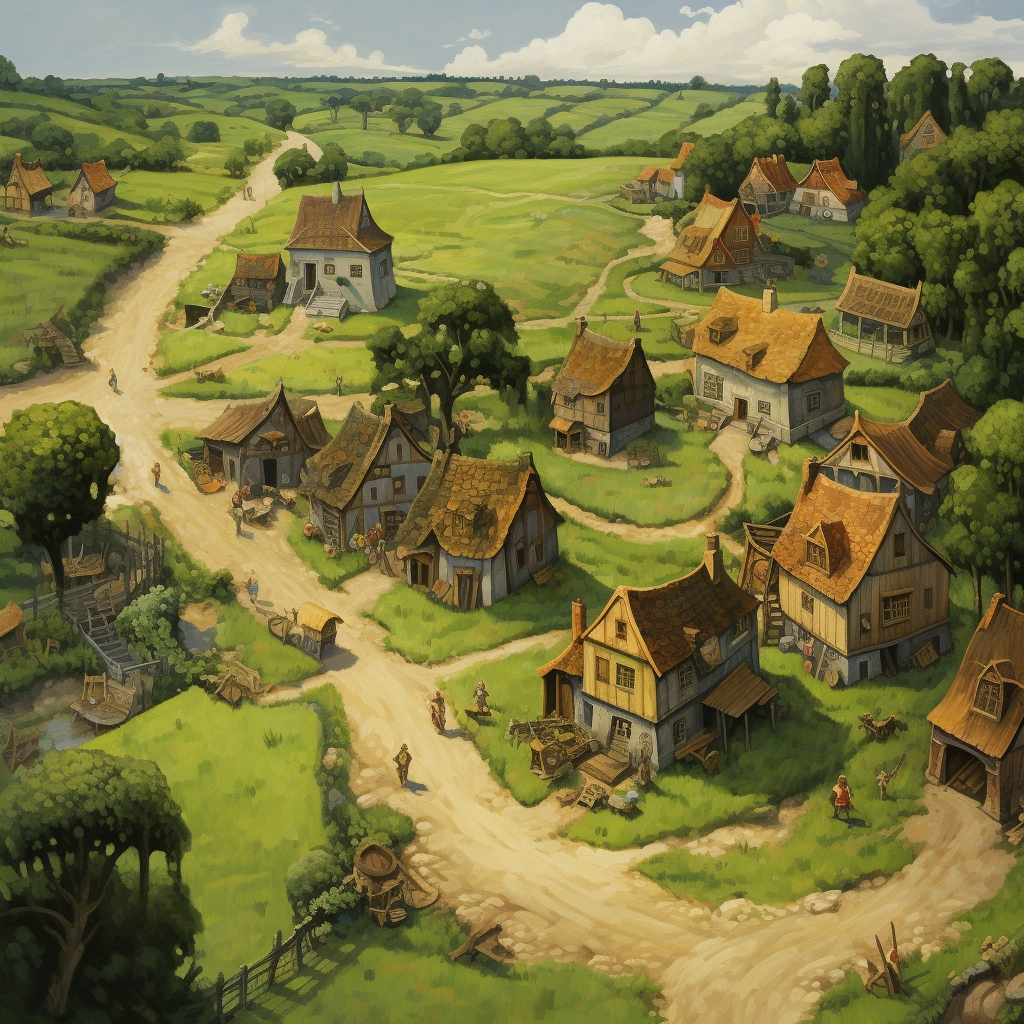
\includegraphics[scale=0.2]{BilderFuerBA/MeilensteinGebaude/a_scatch_from_a_village_top_down.png}
   		 \caption{a scatch from a village, top down}
   		 \label{fig:Midjourney-Conceptart-Dorf}
\end{figure}
Nach der Erstellung der Hauptspielfigur, ist der nächste Schritt das Erstellen einer Spielwelt.
\\
Die Idee ist es, ein Dorf in der Unreal Engine 5 zu erschaffen. In diesem Dorf befinden sich verschiedene Gebäude.
\\
In diesem Kapitel möchte ich zeigen, wie ich die Gebäude mit Hilfe verschiedener KI-Systeme in der Unreal Engine 5 realisiert habe. Ich werde in diesem Kapitel und in den folgenden Meilensteine nicht mehr so detailliert alles wie bei der Erstellung der Hauptfigur, sondern nur auf Schritte eingehen, die im Prozess unterscheiden.
\\
Fachwerkhäuser repräsentieren etwas Mittelalterliches, und da die Renaissance an das Mittelalter zeitlich gegliedert ist, waren in Zeiten der Renaissance Fachwerkhäuser sehr weit verbreitet.
\\
Meine Idee ist es, Diverse Fachwerkhäuser zu erschaffen und auf einer Landschaft zu verteilen, um eine Dorflandschaft zu kreieren.
\\
Mein erster Ansatz ist es, Häuser mit Hilfe von einem einfachen 3D-Modell umzusetzen, was ich in Blender erstellt habe. Dieses 3D-Modell bestand aus einem Quader mit einer Spitze. Kurz, ein einfaches Haus.
\\
Mit Midjourney habe ich Texturen erstellt, die Fachwerkhäuser nachempfunden sind. Diese Texturen und das einfache Haus wurden mit Hilfe von Blender verbunden.
\\
Folgend wurden die einfachen Fachwerkhäuser in Unreal Engine 5 Importiert und verteilt.
\\
Die erste Ansatz funktioniert, bringt aber ein Problem mit sich - die Modelle wirken etwas platt und langweilig.
\\
Besonders da die Kamera sich direkt hinter der Spielfigur befindet und frei schwenkbar ist. Anders, wenn die Kamera so angeordnet ist, wenn sie nur von oben herab schaut. Dafür wären solche Modelle wiederum sehr gut geeignet.
\\
Dieser Ansatz ist nicht gut geeignet, denn die Hauptfigur bewegt sich in der Third-Person durch die Spielwelt. Das Problem mit der Third Person ist, dass man Objekte sehr nah betrachten kann und dadurch unschöne Modelle eher  negativ auffallen als zum Beispiel in der Top-Down-Perspektive, wo 3D-Modelle nur von oben zu betrachten sind.
\\
Eine Inspiration für meinen zweiten Ansatz ist Valheim, ein Survival-Spiel von den Coffee Stain Studios. In diesem Spiel gibt es ein Baukastensystem, in dem der Spieler sein eigenes Haus bauen kann.
\\
In Valheim kann der Spieler verschiedene Wände, Balken, Fußböden, Dächer und Materialarten auswählen, um damit seine Behausung zu gestalten.
\\
Hinzu kommen andere Elemente wie Zäune und Gemüse um ein Garten zu erschaffen, Werkbänke, Tische und Stühle um eine Inneneinrichtung zu kreieren und sogar Teppiche aus Tierfelle und Trophäen die man an die Wand hängen kann um eine Dekorative charakter in die Behausung eines Spielers zu schaffen.
\\
Aus dieser Inspiration habe ich einen zweiten Ansatz entwickelt und zwar einen so genannter Dorfbaukasten.
\\
Dieser Dorfbaukasten besteht ebenfalls aus Wänden, Balken, Dächer, Fußböden und Tapeten.
\\
Im Grunde genommen besteht ein Fachwerkhaus auch aus simplen Bauteilen, wie zum Beispiel Wände, Balken, ein Dach, Türen und Fenster. Diese einzelnen Elemente möchte ich nachbauen, so dass man im Unreal Engine Editor ein Haus selber bauen kann.
\\
Ziel ist es, diese einzelnen Elemente zu programmieren, damit die Materialeigenschaft sich untereinander unterscheiden. Zum Beispiel wirkt jeder Balken unterschiedlich, weil durch Midjourney fünf unterschiedliche Holzmaterialien erstellt wurden.
\\
Mein erster Ansatz war gut, aber nicht gut genug. Ich habe mich als ein Mann Videospiel Entwicklung gegen meinen ersten Ansatz entschieden. Nach der Implementierung in der Unreal Engine 5, sahen die 3D-Modelle für mein Geschmack etwas zu plastisch und platt aus. Die Balken innerhalb. Des Fachwerks haben keine Schatten geworfen und.  Sah einfach zu künstlich aus für meinen Geschmack. Also habe ich einen zweiten Ansatz entwickelt. Der zweite Ansatz besteht aus einem Baukastensystem, jeder Balken, jede Wand und jedes Dachelement hat.  Eine eigenes Element.  Diese Elemente können kann ich die diese Elemente, die in der Regel aus. Einfachen Formen wie?
 
Quader, oder? Dreiecke bestehen.  Kann ich einfach mit einem blueprint Skript.  Die Texturen jeweils. Hinzufügen.  Das bedeutet, ich brauche keinen Blender mehr, um ein 3 D Modell zu erzeugen, sondern mit einfachen.  Formen. Geometrien. Die über die andere Engine.   Mir zur Verfügung gestellt werden.  Mir einen einfachen Bausatz erstellen kann, die ich dann zusammengesteckt. Zusammenstecken kann. Um halt einfache Fachwerkhäuser. Zu erstellen.  Der Vorteil meines zweiten Ansatzes liegt darin, dass ich. Individuellere. Gebäude erstellen kann.
 
Die Sicherheit. Klar, auch in Form.  Von den Nachbarnhäusern unterscheiden. 	 Ein weiterer Vorteil ist, ich kann Innenräumen gestalten, das in der ersten Version nicht. Möglich gewesen ist. Oder möglich ist.   	 Ich kann mit der zweiten Version Innenräumen auch Fußboden gestalten. Ich kann Tapeten gestalten.
 
\subsection {Meilenstein: Nebenfiguren}
Beim dritten Meilenstein Nebenfiguren möchte ich gerne beschreiben, wie ich meine Nebenfiguren, kurz NPCs, erstellt habe. Ähnlich wie beim Erstellen der Hauptfigur habe ich durch Chat GPT mir verschiedene NPCs beschrieben lassen. Zu dieser Beschreibung gehörte Alter, Geschlecht, Beruf unnd charakterliche Eigenschaften.
\\
Mit diesen Beschreibungen habe ich mir einen Prompt mit hilfe der Midjourney-Formel überlegt und Midjourney hat mir Conceptgraphiken erzeugt. Nach mehreren Versuchen habe ich zwei Conzeptgraphiken bekommen die ich für PIFuHD verwenden kann.
\\
Nach dem ich PIFuHD die beiden Conzeptgraphiken übergeben habe, wu rden sie Wie bei der Hauptfigur in Blender der Polycount reduziert und Texturiert.  Stark verformete stellen die an den Händen und Füßen auftreten wurden im Eddit Mode, oder im Sculp Mode nachgebessert.
\\
Für den Prototyp impotiere ich die NPCs ohne Sceleton Mesh ein, da sie keine Laufanimation benötigen, sonder nur in der Spielwelt plaziert werden um mit dem Hauptcharakter zu reden.
\\
Dadurch das die NPC keine Sceleton Mesh besitzen ist auch gut zu erkennen, das die NPCs keine großen verformungen aufweisen wie die Hauptfigur. Die Verformung tritt z. B. in bereich der Hüfte sehr stark auf aufgrund der unterschiedlich gewichtete zuweisung der Vertices zu den einzelen Bones des Sceleton Mesh.


%\\\\\\\\\\\\\\\\\\\\\\\\\\\\\\\\\\\\\\\\\\\\\\\\\\\\ Dialogsystem\\\\\\\\\\\\\\\\\\\\\\\
%\\\\\\\\\\\\\\\\\\\\\\\\\\\\\\\\\\\\\\\\\\\\\\\\\\\\ Dialogsystem\\\\\\\\\\\\\\\\\\\\\\\
%\\\\\\\\\\\\\\\\\\\\\\\\\\\\\\\\\\\\\\\\\\\\\\\\\\\\ Dialogsystem\\\\\\\\\\\\\\\\\\\\\\\
\subsection {Meilenstein: Dialogsystem}
Um ein Dialogsystem in der Unreal Enginge 5 zu entwickeln habe ich mehrere Ansätze gebraucht.
 
Ansatz 1 mit ChatGPT
Ich habe ChatGPT dazu Aufgefordert mir ein Dialogsystem zu entwickeln damit mein Hauptcharakter mit den NPCs aus meinem Prototyp sich unterhalten können.
 
Ich habe versucht die Schritte umzusätzen die ChatGPT mir vorgegeben hat – Erfolglos.
 
Ansatz 2 Rechersche mit Suchmaschienen im Internet
Mit der Suchmaschiene Google
Durch Google bin ich auf ein Video auf Youtube gestoßen, was mir erklärt hat wie ich ein Dialogsystem in Unreal Engine 5 erstellt wird.
\\
Zu dem beschreibenen Dialogsystem wurde von mir noch ein Dilay in der Länge von dem Soundfile hinzugefügt und ein Bool, der auf false steht, falls eine Interaktion gerade nicht möglich ist, zu beispiel ein Charakter redet gerade noch. Dieser Bool soll verhindern, damit keine Dialoge schnell hintereinander gestartet werden und die Charaktere aussprechen lässt.
\\
Um die Sprachausgabe zu managen, braucht es ein Dialogsystem. Für das Dialogsystem habe ich
versucht, eine art Dialog System zu erschaffen, das man zum Beispiel aus der Sincefiction Spielereihe Mass Effect kennt. In dem der Spieler verschiedene Antworten- oder Fragemöglichkeiten besitzt. Das hat leider nicht von seiten ChatGPT nicht geklappt.
\\
Ich habe auch ChatGPT gefragt, wie ich ein Dialogsystem in der Unreal Engine 5 umsetzen kann. Auch das hat leider nicht funktioniert.
\\
An dieser Stelle ist gut zu erkennen das KI-Tool sehr gute ergebnisse erzeugen kann um ein Videospielprototypen zu entwickeln, aber KI-Systeme haben ihre Grenzen, sowie ich Als Ein-Mann-Videospiele-Entwickler auch grenzen habe in der Kompetenz diese Systeme zu bedienen.
\\
Das Problem, dass ich nicht weiß wie ein Dialogsystem entwickelt wurde, und ChatGPT mir ein Falsche lösung mir überreicht hat, habe ich durch die Suchmaschiene von Google und Youtube ein Tutorial gefunden wie ich ein Dialogsystem zwischen meiner Hauptfigur und den NPCs entwickeln kann.
\\
Also habe ich gegoogelt und auf youtube ein Tutorial gefunden.  	 Mit der andere Engine 5. Musste ich eine Schnittstelle, was zwischen den verschiedenen.  Actors wie zum Beispiel der Hauptfigur und den MPC.  Eine Schnittstelle bildet.    		 Diese Schnittstelle habe ich mit Blueprince umgesetzt. Ich musste auch bei blueprint m bei meiner Hauptfigur Martin Luther.  	 Etwas entwickeln und zwar habe ich ein Array erzeugt oder mehrere Arrays erzeugt. Die speichert, was gesagt wird, in Schriftform und was gesagt wird in.   Ausgabe.  In Sprachausgabe, in Soundausgabe.
\\
Ich habe eine Aktionsbutton hinzugefügt, was für was in diesem Beispiel der Buchstabe auf der Tastatur e ist.  Der sagt, Hey, ich möchte mit dir arbeiten.		 Ich habe einen Pool A erzeugt, die. Signalisiert. Hey, ich kann jetzt interagieren mit der Person oder gerade nicht.   		 Da das Dialogsystem. Vor z GPT unvollständig war habe ich mir noch andere Dialog Dialoge hinzu ausgedacht, andere Dialoge ausgedacht.  Und somit war das Dialogsystem auch schon fertig.



%\\\\\\\\\\\\\\\\\\\\\\\\\\\\\\\\\\\\\\\\\\\\\\\\\\\\ Sprachausgabe\\\\\\\\\\\\\\\\\\\\\\\
%\\\\\\\\\\\\\\\\\\\\\\\\\\\\\\\\\\\\\\\\\\\\\\\\\\\\ Sprachausgabe\\\\\\\\\\\\\\\\\\\\\\\
%\\\\\\\\\\\\\\\\\\\\\\\\\\\\\\\\\\\\\\\\\\\\\\\\\\\\ Sprachausgabe\\\\\\\\\\\\\\\\\\\\\\\
\subsection {Meilenstein: Sprachausgabe}
Nachdem ich das Dialogsystem erstellt und implementiert habe, fehlt nur noch der Inhalt, was die Charaktere miteinander als sich erzählen. Und zwar habe ich hier zwei neue Ki-Systeme benutzt, die vorher noch nicht zum Einsatz gekommen diese sind Voice AI und Adobe Enhance Speache.
\\
Voice AI ist ein KI-System, die Stimmen verändern kann. Zum Beispiel kann man seine Stimme so manipulieren, das sie wie die von Kanye West oder dem amtierende US-Präsident Joe Biden klingt.
\\
Adobe Enhanced ist ein KI-System, das deine gesprochene Stimme so klingen lässt, dass sie in einem hochwertigen Tonstudio aufgenommen wird.
\\
Meine Sprachaufnahmen verwende ich das Mikrofon von dem Logitech G35 Headset was seit 2014 nahezu täglich benutz wird.
\\
Durch die Kombination von Adobe Enhance Speech und Voice AI habe ich qualitativ hochwertige Sprach Dateien erzeugen können, die sonst ein hochwertiges Tonequipment und gute Dämmung in meinem Büro erzeugt hätten.
\\
Um die Stimmen für die NPCs zu erzeugen, habe ich drei verschiedene Experimente durchgeführt.
\\
\subsubsection{Erst Adobe Enhance Speache dann Voice AI}
Als erstes wurde der Klang meiner stimme mit Audacity und meinem Logitech G35 Headset aufgenommen.
\subsubsection{Erst Voice Ai dann Adobe Enhance Speech}
\subsubsection{Erst Adobe Enhance Speech dann Voice AI dann wieder Adobe Enhance Speech}
 
Experiment eins, erst Voice I gegeben und dann Adobe Anshan Speech. 		 Oder? Erst Adobe, Assange Speech und dann Voice AI.  Ich habe noch eine dritte.
\\
Variante ausprobiert, und zwar eine Art Sandwich Methode, indem ich meine Sounddatei, die ich mit Audacity aufgenommen habe, erst Adobe 1. Hand speech. Dann Voice I und dann wieder Adobe A Speech gegeben habe, um so eine Art zweifache Reinigung. Der Sprache oder der Sprachausgabe zu erhalten.     Mein persönliches bestes Ergebnis, was auch Zeittechnisch am. Sparsamsten war.  Ist erst.  Athan Speech zu benutzen und dann Voice I. Die dritte Version ist auch ok, aber es kann sein, dass danach sich die Stimme noch etwas künstlicher, Blecherner anhört.   Generell ist die Sprachausgabe sehr.  Gut.
\\
Und professionell anwendbar für mein Prototyp ist das eine Qualität, die ich früher nicht erreicht hatte können außer mit großen Aufwand und Kosten verbunden wie ZB das Kaufen eines 200€, Mikrofons und sehr guter Dämmung in meinem Aufnahmeraum. Ich habe die Aufnahmen bei einem sonnigen Tag während. Traktoren im Hintergrund arbeiten. Ich habe in meinem Arbeitszimmer. Ein Fenster aufgehabt. Das offenbar zu einem Bauernhof in meiner Nachbarschaft. Man kann Traktoren hören, man kann meine Frau hören, im Hintergrund, die in der Wohnung mit den Kindern sich beschäftigen und anhand Speech hat das alles herausgefiltert. Und ein gewisses Grundrauschen befindet sich auch nicht mehr und der Sound-Datei.
\\
Die Meilensteine.  Die ich hier in meiner Bachelor thesis beschreibe.  Sind nicht chronologisch sortiert, sondern nur logisch.  Ich habe das Dialogsystem und die Sprachausgabe gleichzeitig entwickelt und.  Implementiert.  Die Sprachausgabe, die ich hiermit mit Voice I und Adobe anhand Speech. Geschaffen habe, habe ich nun in das.  Dialogsystem was sich in dem vorigen Kapitel beschrieben habe. Implementiert. Ich habe die Sprachausgabe in das Array getan.		 In der andere Engine 5.
 
\subsection{Erstellung von Musik und Klängen}
\subsection{Erstellung von Animationen}
\subsection{Entwicklung der Spiellogik}
%5
\section{Ergebnisse und Diskussion}
\subsection{Vorstellung des fertigen Videospiels}
 
\subsection{Diskussion der Ergebnisse und Einschätzung des Erfolgs des KI-Einsatzes}
\subsubsection{Einsatz von MonsterMash}
Monster Mash ist ein KI-System, mit dem man Monster erstellen kann. Wenn man sich realitätsnahe Ergebnisse wünscht, wird man mit Monster Mash auf sehr große Herausforderungen treffen.
\\
Monster sind Fantasiewesen, und niemand kann genau beschreiben, wie ein Monster aussieht. Bei der Darstellung von Menschen oder Gebäuden sieht das anders aus. Für mein Adventure-Game, mit einem historischen Hintergrund, ist MonsterMash nicht zu empfehlen.
\\
Anders würde es in einem Fantasy-Szenario aussehen, wo undefinierte Gestalten dem Spieler begegnen sollen.
\subsubsection{Einsatz von PFuHD}
PIFuHD ist eine KI-System was darauf trainiert ist, Digitalfotos von Personen in ein 3D-Modell umzuwandeln. PIFuHD kann man auf Google-Collab einrichten und lauffähig machen.
\\
Für das erstellen von 3D-Modellen wurde PIFuHD ist in der kostenlosen Demo-Version verwendet.
\\
Die Kompatibilität zwischen Midjourney und PIFuHD ist möglich. Die Resultate sind zum teil Artefakt belastet, die besonders in Bereichen der Hände, Füße und Kleidung auftreten.
\\
Durch Midjourney konnte ich Bilder von Martin Luther erzeugen, die als Konzeptgrafiken dienten. Diese Konzeptgrafiken habe ich PIFuHD als eingabe gegeben, und hat mir daraus folgende 3D-Modelle von Personen ausgegeben, die im Prototyp als Hauptfigur und NPCs verwendet wurden.
\subsection{Kritische Reflexion des Entwicklungsprozesses und Ausblick auf mögliche zukünftige Entwicklungen}

\section{Allgemeine Probleme mit KI und KI-Systeme}
Ich möchte an dieser Stelle auf eine Auswahl gesellschaftliche Punkte eingehen, die mich während meiner Arbeit mit und über KI-Systeme begegnet sind und mich als Ein-Mann-Videospielentwickler begleitet haben.
\subsection{KI-Systeme und ihrer Monatarisierung}%steam verbietet verkauf von ki-asset speiele
\subsection{KI-Systeme und ursachen auf andere Berufe}%entwickler in china entlässt concet artist um selber mit ki-systemen wie midjourney zu arbeiten
\subsection{Ki-Systeme und der Biologischer Fussabdruck}%ki-systeme verbrauchen viel strom um sie zu trainieren
\subsection{KI-Systeme aund die auswirkung als Entwickler}%wahrscheinlich persönlich was ich immer gedacht habe immer ki immer ki und weniger selber nachdenken.. man sollte auch vertrauen auf seine fähigkeiten haben, oder auf seine menschliche gesellschaft hilfe suchen. es icht nicht schlimm ein musiker nach musik zu fragen, und zu bezahlen.
\subsection{Dritte-Welt länder vs. Erste-Welt länder}%ki-systeme werden offt in schwellenländer trainiert für ein hungerlohn
\subsection{Firmeninteressen} %die entwickler solcher ki-systeme haben eigene interessen wie Politik china und tiktok.. china klavier usa gefährliche chellenges
\subsection{Geistiges eigentum}%zum beispiel JR-Tolkin un die US-Schriftsteller verband verkagen OpenAI da sie Texte zum Trainieren benutzen ohne zustimmung, genau so wie berühmte Digital Artist in steal von  Studio gibli und kuvshinov digital artist die über jahrzehnte ihren stil entwicklet haben

%6
\section{Fazit}

Fragestellung: Welche Möglichkeiten bieten KI-Systeme einem Ein-Mann-Videospieler bei der Entwicklung eines Videospiels?  

In dieser Arbeit wurde der Frage nachgegangen, welche Möglichkeiten KI-Systeme einem Ein-Mann-Videospieler bei der Entwicklung eines Videospiels bieten. 

Anhand der Entwicklung meines Prototypen, habe ich herausgearbeitet, dass ….


KI-Systeme laden zum Experimentieren ein. Als Ein-Mann-Videospieler ist es möglich, einen Plot für Videospiele in Minuten zu schreiben, wofür ich Wochen benötigen würde und das nur durch einen einfachen Prompt für ChatGPT.
\\
Ich kann Konzeptgrafiken, UX-Elemente, Texturen in Hülle und Fülle mit Midjourney generieren, ohne nur einen Stift oder Grafiktablett in die Hand zu nehmen.
\\
Als Legastheniker und untalentierter Maler und Zeichner bieten mir KI-Systeme noch nie da gewesene Möglichkeiten, mich kreativ auszuleben.
\\
Die in Kapitel 5 verwendeten KI-Systeme sind nur ein Beispiel, mit denen ich gute und sinnvolle Ergebnisse für meinen Prototyp erstellt habe. Ich habe mich mit vielen weiteren KI-Systemen beschäftigt und diese ausprobiert, die aber in der Entwicklung meines Prototypes keinen Einfluss hatten.
\\
KI-Systeme wie zum Beispiel MonsterMash, mit dem man mit einem Hintergrundbild und einer Zeichnung mit der Maus ein einfaches 3D-Modell erzeugen kann. Dieses 3D-Modell kann man mit Hilfe von bewegbaren Punkten animieren.
\\
Ich habe die Photoshop-KI von Adobe ausprobiert. Mit diesem KI-System konnte ich zum Beispiel die Texturen, die ich für mein einfaches Haus von Midjourney bekomme, so bearbeiten, dass aus einer Tür ein Fenster wird.
\\
Ich wollte mit einem KI-System namens Kaedim arbeiten, da sie einer der wenigen KI-Systemen die fähigkeit besaß, aus Bildern 3D-Modelle zu erzeugen. Der Preis von circa 15€ pro Prompt hat mich abgeschreckt. Hinzu kam das Kaedim eine sehr lange bearbeitungszeit benötigt hätte, von ca 20 Minuten war die Rede, was ich in diesem Moment sehr Merkwürdig fand.
Durch ein Blick in der Dokumentation, wurde Kaedim so beschrieben, das es eine Mischung aus einem Trainierten KI-System und 3D-Artist ist, von dem ich das Ergebnis bekommen würde.
Da ich mich als Ein-Mann-Videospielerentwickler sehe, habe ich mich dazu entschieden, dieses KI-System zu verwenden, da ich erstmal keinen anderen Menschen an meinem Prototyp arbeiten lassen möchte.
\\
Ich habe mich auch auf Soundful Music und AIVA angemeldet und versucht in Richtung Music zu forschen und Experimentieren, aber meine Zeit das leider nicht zugelassen.
\\
Musik finde ich ein Spannendes gebiet, und es gibt KI-Systeme die sich in diesem Thema sich bewegen. Leider hatte ich keine zeit im Rahmen meiner Bachelorthesis mich in dieser Richtung intensiv zu experimentieren.
\\
Während meiner Projektphase hatte ich immerwieder das gefühl, das das Wort KI und AI oft als Marketing buzzwort benutz haben um sich vom Markt abzuheben.
\\
KI-Systeme zu erforschen und erfahren, kann sehr viel zeit in Anspruch nehmen. Mit jedem Neuen System muss man üben. Jedes KI-System hat grenzen die die Erwartungen oder Anforderung eines Ein-Mann-Videospieleentwickler entsprechen.
\\
Ich möchte in diesem Fazit ein wenig bildlich werden.
\\
Wenn ein Videospiel Prototyp ein dreistöckiges Haus wäre:
Das Fundament, der Keller und alle Leitungen wie Wasser, Strom und Gas ist die Unreal Engine 5.
Der Erste- sowie die Hälfte des Zweiten-Stocks, der größte Teile der Außen- und Innenfassade, können Ergebnisse von KI-Systemen sein.
Der Rest hängt von dem Ein-Mann-Videospielentwickler und seinen Fähigkeiten ab um ein schlüsselfertiges Haus zu bauen.
\\
Mein Prototyp hat eine erkennbare Form, ist aber noch weit davon entfernt um Potenzielle Geldgeber, wie die Deutsche Gameförderung, zu überzeugen um mich als Ein-Mann-Videospielentwickler Geld zu bekommen um aus meinem Prototyp ein Fertiges, marktreifes Spiel zu erschaffen.
\\
Mein Ziel war es, Inhalte für mein Prototyp mit Hilfe von KI-Systemen für die Unreal Engine 5 zu erschaffen, und ich bin So
\subsection{Zusammenfassung der Ergebnisse}
\subsection{Implikationen für die Praxis}
\subsection{Limitationen der Studie}
%7
\section{Literaturverzeichnis}
\printbibliography
%8
\section{Anhang}
\subsection{Abbildungen und Diagramme}
\subsection{Code-Beispiele}
\printbibliography

\subsection{Weitere Materialien}

%

\end{document}
 
 
%erklärungen wie welche programme eingerichtet und benuttz werden können als Anhang hinzugefügt werden

%hallo test eins



%\subsection{Nutzung von KIs zur Erstellung von 2D Bildern}
%Als erstes brauche ich eine Spielfigur die Martin Luther nachempfunden ist. Mein Worklfow besteht darin ein Promt von ChatGPT ausgeben zu lassen, den ich Später für Midjourney benutzen kann. Genau diesen Prompt habe ich ChatGPT übergeben.

%\begin{figure}[h]
%    \centering
%    \begin{minipage}[t]{0.45\linewidth}
%   	 \centering
%   	 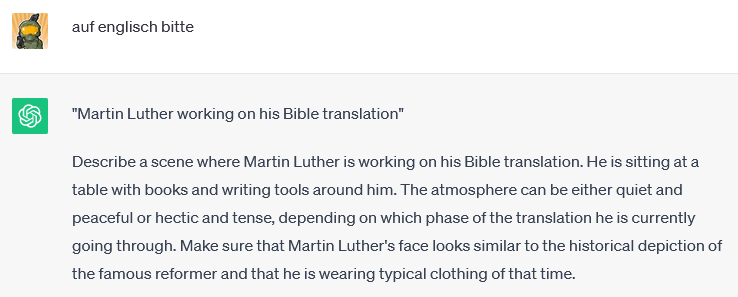
\includegraphics[width=7cm]{BilderFuerBA/CGPTMidJourneyMartinLuther/03.png}
%   	 \caption{Dritter Versuch: ChatGPT erstellt Promt für Midjourney in Englisch}
%    \end{minipage}
%    \hfill
%    \begin{minipage}[t]{0.45\linewidth}
%   	 \centering
%   	 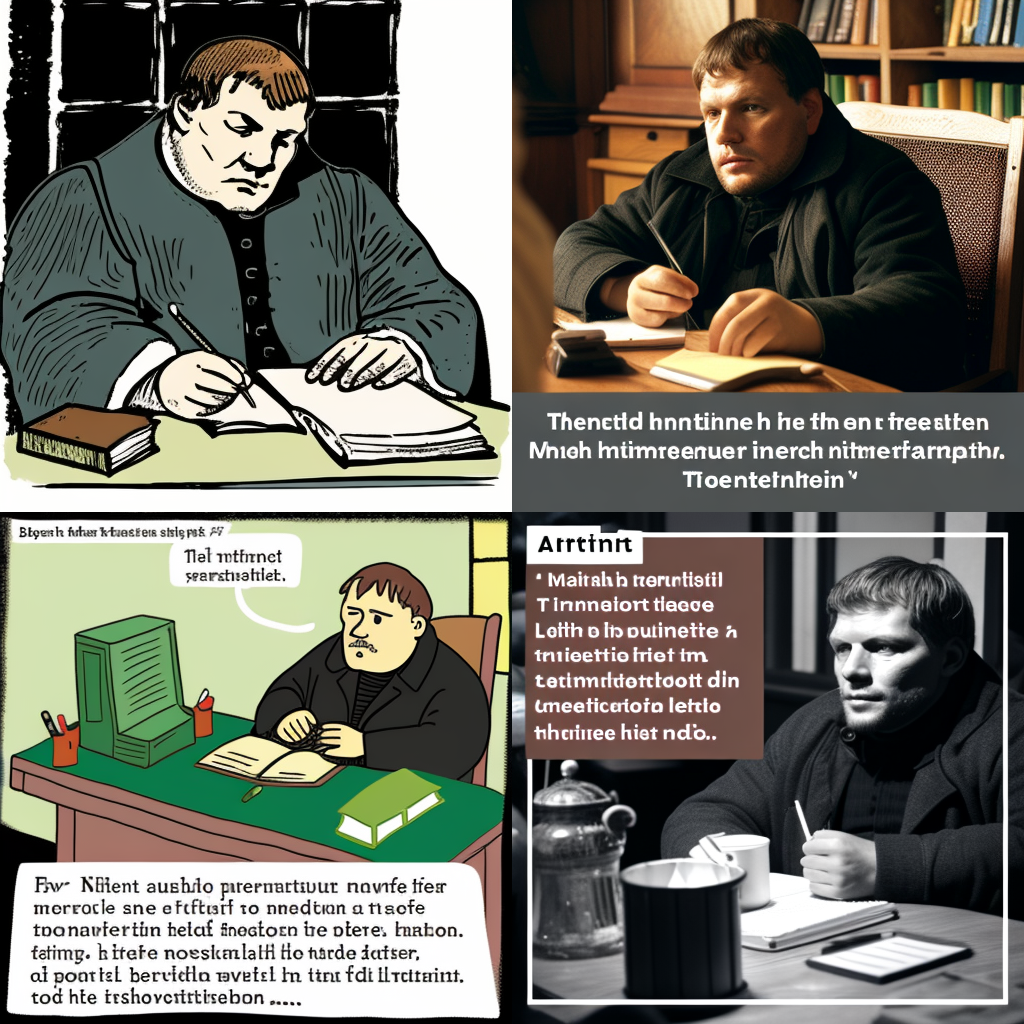
\includegraphics[width=7cm]{BilderFuerBA/MJ/MLaufEnglisch.png}
%   	 \caption{Describe a scene where Martin Luther is working on}
%    \end{minipage}
%   	 
%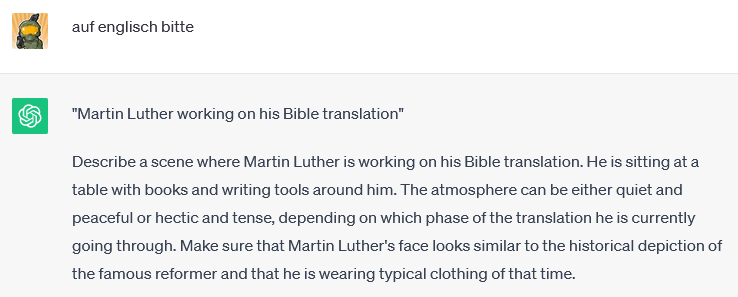
\includegraphics[scale=0.7]{BilderFuerBA/CGPTMidJourneyMartinLuther/03.png}
   		 ´%\caption{Dritter Versuch: ChatGPT erstellt Promt für Midjourney in Englisch}
   		 %\label{fig:chatgpt-ptompt-Midjourney-03}
%\end{figure}
%\end{figure}    \begin{figure}    \centering    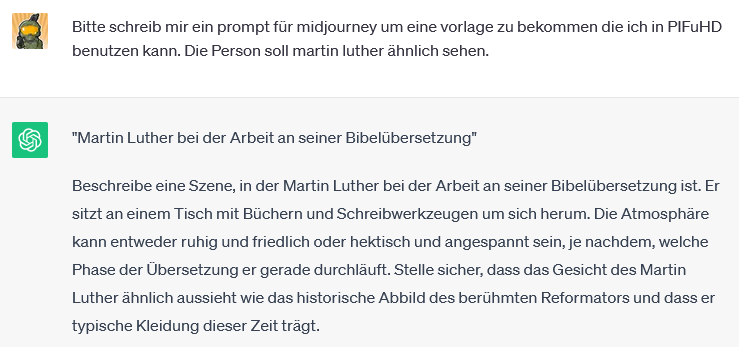
\includegraphics[width=14cm]{BilderFuerBA/CGPTMidJourneyMartinLuther/02.png}    \caption{Zweiter Versuch: ChatGPT erstellt Promt für Midjourney ohne Rechtschreibfehler}    \label{fig:chatgpt-ptompt-Midjourney-02}\end{figure}


